%% 
%% This is a sample doctoral dissertation.  It shows the appropriate
%% structure for your dissertation.  It should handle most of the
%% strange requirements imposed by the Grad school; like the different
%% handling of titles of one/many appendices.  It will automatically
%% handle the linespacing changes.  The body default is double-spaced
%% (except when you use the singlespace or condensed options).  The
%% default for quotations is single-space, and the default for tabular
%% environments is also single-space.  
%%
%% This class adds the following commands and environments to the
%% report class, upon which it is based:
%% Commands
%% ------------
%% \degree{name}{abbrv} -- Sets the name and abbreviation for the degree.
%%                         These default to ``Doctor of Philosopy''
%%                         and ``Ph.D.'', respectively.
%% \copyrightyear{year} -- for the copyright page.
%% \bachelors{degree}{institution} -- for the abstract
%% \masters{degree}{institution}   --  "
%%     if you have other degrees you may use
%% \secondbachelors{degree}{institution}
%% \thirdbachelors{degree}{institution}
%% \secondmasters{degree}{institution}
%% \thirdmasters{degree}{institution}
%% \priordoctorate{degree}{institution}
%%
%% \committeechair{name}           -- for the signature page
%% or, if you have two co-chairs:
%% \cochairs{first name}{second name}
%%
%% \firstreader{name}              --  "
%% \secondreader{name}             --  "
%% \thirdreader{name}              -- (optional)
%% \fourthreader{name}             --  "
%% \fifthreader{name}              --  "
%% \sixthreader{name}              --  "
%% \departmentchair{name}          -- for the signature page
%% \departmentname{name}           --  "
%%
%% \copyrightpage                  -- produces the copyright page
%% \signaturepage                  -- produces the signature page
%%
%% \frontmatter                    -- these are required in their various
%% \mainmatter                     -- appropriate locations
%% \backmatter                     --
%%
%% \unnumberedchapter[toc]{name}   -- like \chapter, except that it
%%                                    produces an unnumbered chapter;
%%                                    alternatively, like \chapter*,
%%                                    except that it lists the chapter
%%                                    in the table of contents.
%%
%% New environments:
%%   dedication  -- for the dedication
%%   abstract    -- for the abstract
%%
%% The thesis documentclass is built on top of the report document class.
%% It accepts all of the options that the report class accepts, plus the
%% following:
%%     doublespace -- the default, indicates double spacing as per U.Mass.
%%                    requirements.  You will need this when you do your
%%                    final copy.
%%     singlespace -- for earlier work, not acceptable to the Grad school
%%     condensed   -- for earlier work, not acceptable to the Grad school,
%%                    creates condensed versions of the frontmatter. 
%%                    Condensed implies singlespace.
%%     dissertation - the default, indicates that this document is a
%%                    dissertation.
%%     proposal    -- indicates that this document is a dissertation proposal,
%%                    rather than a dissertation.  This will only change the
%%                    wording on the title and signature pages.
%%     thesis      -- indicates that this document is a Master's thesis 
%%                    rather than a doctoral dissertation.  This also changes
%%                    the default for \degree to Master of Science, M.S.
%%     allowlisthypenation -- (the default), allows hyphenation of words in
%%                    the table of contents, the list of figures, and the list
%%                    of tables.  I believe that this is acceptable to the 
%%                    Graduate School.
%%     nolisthyphenation -- disallows hyphenation of words in the table of
%%                    contents and the list of figures and tables.  Use this 
%%                    option if the Grad School doesn't like your hyphenation.
%%     nicerdraft  -- relaxes some of the Grad School's rules for working with
%%                    drafts -- has no effect when doublespace is in effect
%%     nonicerdraft -- the default, leaves things in draft as they will be in
%%                     the final version
%% umassthesis changes the default font size to 12pt, but you may specify 10pt or
%%   11pt in the options.
\documentclass[proposal,singlespace]{umassthesis}          % for Ph.D. dissertation or proposal
% \documentclass[thesis]{umassthesis}  % for Master's thesis

%%
%% If you have enough figures or tables that you run out of space for their
%% numbers in the List of Tables or List of figures, you can use the following
%% command to adjust the space left for numbers.  The default is shown:
%%
%% \setlength{\tablenumberwidth}{2.3em}

%% Use the hyperref package if you're producing a version for online
%% distribution and you want hyperlinks.  Note that the Grad School doesn't want
%% their PDF viewers to colorize or otherwise highlight the links; use the
%% hidelinks option to hyperref to avoid decorating links.
%\usepackage[hidelinks]{hyperref}

%% One way of formatting the epigraph/frontispiece is to use this package.
%\usepackage{epigraph}


\usepackage{verbatim}


%vertex connectivity preamble stuff

\usepackage{url}
%\usepackage{color,fullpage,microtype}
%\usepackage{graphicx,wrapfig,subfigure,titling}
\usepackage{amssymb,amsmath,amssymb,amsfonts}
\usepackage{amsthm}
\usepackage{textcomp}
\usepackage{multirow}
%\usepackage{gensymb}
\usepackage{array}
\usepackage{times}
\usepackage[sort]{cite}

\newtheorem{theorem}{Theorem}%[section]
\newtheorem{definition}[theorem]{Definition}

\newtheorem{proposition}[theorem]{Proposition}%[section]
\newtheorem{corollary}[theorem]{Corollary}%[section]
\newtheorem{lemma}[theorem]{Lemma}%[section]
\newtheorem{conjecture}[theorem]{Conjecture}%[section]
\newtheorem{fact}{Fact}
\newtheorem{problem}{Problem}
%\newtheorem{example}{Example}
\newtheorem{claim}{Claim}

%\newcommand{\vecx}{\mathbf{x}} 
\newcommand{\vecy}{\mathbf{y}} 

\newcommand{\expec}[1]{\mathbb E\left [ #1 \right ]}
\newcommand{\rounddown}[1]{\left \lfloor  #1 \right \rfloor}
\newcommand{\roundup}[1]{\left \lceil  #1 \right \rceil}
\DeclareMathOperator{\polylog}{polylog}
\DeclareMathOperator{\poly}{poly}
\DeclareMathOperator{\light}{{light}}
%\DeclareMathOperator{\outdeg}{out-deg}
%\newcommand{\inneigh}{\Gamma^-}
%\newcommand{\outneigh}{\Gamma^+}

\newcommand{\todo}[1]{{\color{blue}[\textit{#1}]}}
\newcommand{\reals}{{\mathbb R}}
\newcommand{\prob}[1]{\mathbb P \left [ #1 \right ]}
%\newcommand{\Egt}{U}
%\newcommand{\Eslt}{D}

\newcommand{\vecf}{\mathbf{f}} 

%\newcommand{\sfv}{\begin{proof}See full version.\end{proof}}
\newcommand{\sfv}{}
\newcommand{\R}{{\mathbb R}}
\renewcommand{\H}{{\cal H}}
\renewcommand{\O}{{\cal O}}
\newcommand{\etal}{{et al.~}}
\newcommand{\rk}{\mbox{\sc Rk}}
\newcommand{\hatyi}{\hat{y}_i}
\newcommand{\hatk}{\hat{k}} 
\newcommand{\veca}{\mathbf{a}} 
\newcommand{\veczero}{\mathbf{0}}
\newcommand{\vecone}{\mathbf{1}} 
\newcommand{\vecx}{\mathbf{x}} 
\newcommand{\delc}{{\Delta_C(i)}}
\newcommand{\alg}{{\cal A}}
\newcommand{\obj}{{\cal O}}
\newcommand{\y}{{\mathbf Y}}
\newcommand{\bin}{{\mathbf{Bin}}}
\newcommand{\eat}[1]{}
\newcommand{\acc}{E}
\renewcommand{\k}{\kappa}

\newcommand{\A}{{\cal A}}
\newcommand{\B}{{\cal B}}

\newcommand{\I}{{\cal I}}
\newcommand{\D}{{\cal D}}
\newcommand{\X}{{\cal X}}
\newcommand{\Y}{{\cal Y}}
\newcommand{\Z}{{\cal Z}}
\renewcommand{\P}{{\cal P}}
\renewcommand{\S}{{\cal S}}
\newcommand{\cc}{cc}

\newcommand{\E}{{\mathbf E}}
%\newcommand{\comment}[1]{\marginpar{!!!}[#1]}

\newcommand{\err}{{\mathcal E}}
%\newcommand{\comment}[1]{{\color{red} #1} \marginpar{!!!}}


\newcommand{\pparagraph}[1]{\vspace{0.1in}\noindent{\bf \boldmath #1}}




% mesh preamble stuff

%\usepackage{minted}
%\RequirePackage[outputdir=latex.out,cache=false]{minted}
%\RequirePackage[cache=false]{minted}
\usepackage{listings}
\usepackage{microtype}
\usepackage{hyperref}
\usepackage{xspace}
\usepackage{graphicx}
%\usepackage{url}
%\usepackage{amsmath}
%\usepackage{amssymb}
\usepackage{relsize}
\usepackage{tikz}
\usepackage{clrscode3e}
%\usepackage{amsthm}
\usepackage{color}

\newtheorem{observation}{Observation}%[section]


\newcommand{\sm}{\proc{SplitMesher}\xspace}

%% \setmonofont[Scale=MatchLowercase]{DejaVu Sans Mono}
%% \setmonofont{DejaVu Sans Mono}

\SetTracking{encoding={*}, shape=sc}{0} % No tracking for smallcaps

\newcommand{\Mesh}{\textsc{Mesh}\xspace}
\newcommand{\mesh}{Mesh\xspace}
\newcommand{\ndegree}{\textup{d}} % Command \deg already defined by some dependency
%\newcommand{\comments}[1]{[#1]}


%% Some recommended packages.
\usepackage{booktabs}   %% For formal tables:
                        %% http://ctan.org/pkg/booktabs
%\usepackage{subcaption} %% For complex figures with subfigures/subcaptions
                        %% http://ctan.org/pkg/subcaption
%\captionsetup[subfloat]{font={small,sf}}
% Settings for figures and tables. Figure captions are placed below the figure,
% while table captions are placed above the table. All captions are sans-serif.
%\RequirePackage[font={normalsize,sf,bf}]{caption}
\RequirePackage[font={footnotesize,rm}]{caption}
\RequirePackage[position=bottom]{subfig}
\captionsetup[table]{aboveskip=0.5em, belowskip=0.5em}
\captionsetup[figure]{aboveskip=0.5em, belowskip=0em}
\captionsetup[subfloat]{font={footnotesize,rm}}
\setcounter{topnumber}{2}
\setcounter{dbltopnumber}{2}
\setcounter{bottomnumber}{2}
\setcounter{totalnumber}{4}

\renewcommand{\topfraction}{0.85}
\renewcommand{\dbltopfraction}{0.9}
\renewcommand{\bottomfraction}{0.85}
\renewcommand{\textfraction}{0.07}
\renewcommand{\floatpagefraction}{0.85}
\renewcommand{\dblfloatpagefraction}{0.85}

\setlength{\floatsep}{0.5em plus 0.2em minus 0.2em}
\setlength{\dblfloatsep}{0.5em plus 0.2em minus 0.2em}
\setlength{\textfloatsep}{0.5em plus 0.2em minus 0.2em}
\setlength{\dbltextfloatsep}{0.5em plus 0.2em minus 0.2em}

% Utility packages for floats and tables.
\RequirePackage{float}
\RequirePackage{graphicx}
\RequirePackage{booktabs}
\RequirePackage{multirow}




% PathCache sysname
\newcommand{\sysname}{PathCache}






%unique cover stuff
\newcommand{\uc}{
  \ifmmode
  \mathsf{UniqueCover}
  \else
  $\mathsf{UniqueCover}$
  \fi
  \xspace
}

\newcommand{\mc}{
  \ifmmode
  \mathsf{MaxCover}
  \else
  $\mathsf{MaxCover}$
  \fi
  \xspace
}


\newcommand{\setcover}{
  \ifmmode
  \mathsf{SetCover}
  \else
  $\mathsf{SetCover}$
  \fi
  \xspace
}

\newcommand{\maxcut}{
  \ifmmode
  \mathsf{MaxCut}
  \else
  $\mathsf{MaxCut}$
  \fi
  \xspace
}

\newcommand{\maxbisection}{
  \ifmmode
  \mathsf{MaxBisection}
  \else
  $\mathsf{MaxBisection}$
  \fi
  \xspace
}

\newcommand{\submodular}{
  \ifmmode
  \mathsf{SubmodularMax}
  \else
  $\mathsf{SubmodularMax}$
  \fi
  \xspace
}




\begin{document}

%%
%% You must fill in all of these appropriately
\title{Algorithms for Massive, Expensive, or Otherwise Inconvenient Graphs}
\author{David Tench}
\date{Jun 2020} % The date you'll actually graduate -- must be
                     % February, May, or September
\copyrightyear{2020}
\bachelors{B.Sc.}{Lehigh University}
\masters{M.Sc.}{University of Massachusetts Amherst}
%\secondmasters{M.Ed.}{Antioch College}
%\priordoctorate{M.D.}{University of Never-never-land}
\committeechair{Andrew McGregor}
%\cochairs{B. B. Bahh}{I. M. A. Wolf}
\firstreader{Phillipa Gill}
\secondreader{Cameron Musco}
\thirdreader{Markos Katsoulakis}
%\fourthreader{Mary Lamb}   % Optional
%\fifthreader{}            % Optional
%\sixthreader{}            % Optional
\departmentchair[Chair of the Faculty]{James Allan} % Default uses "Department Chair" as the title. To
% use an alternate title, such as "Chair", use \departmentchair[Chair]{Pete Shearer}
% CICS uses "Chair of the Faculty" as of 2019.
\departmentname{College of Information and Computer Sciences}

%% If your degree is something other than a Ph.D. (for a dissertation), or
%% an M.S. (for a thesis), you will need to uncomment the appropriate
%% following line:
%%
%% \degree{Doctor of Education}{Ed.D.}
\degree{Doctor of Philosophy}{Ph.D.}
%%
%% \degree{Master of Arts}{M.A.}
%% \degree{Master of Arts in Teaching}{M.A.T.}
%% \degree{Master of Business Administration}{M.B.A.}
%% \degree{Master of Education}{M.Ed.}
%% \degree{Master of Fine Arts}{M.F.A.}
%% \degree{Master of Landscape Architecture}{M.L.A.}
%% \degree{Master of Music}{M.M.}
%% \degree{Master of Public Administration}{M.P.A.}
%\degree{Master of Public Health}{M.P.H.}
%% \degree{Master of Regional Planning}{M.R.P.}
%% \degree{Master of Science}{M.S.}
%% \degree{Master of Science in Accounting}{M.S. Acctg.}
%% \degree{Master of Science in Chemical Engineering}{M.S. Ch.E.}
%% \degree{Master of Science in Civil Engineering}{M.S.C.E.}
%% \degree{Master of Science in Electrical and Computer Engineering}{M.S.E.C.E.}
%% \degree{Master of Science in Engineering Management}{M.S. Eng. Mgt.}
%% \degree{Master of Science in Environmental Engineering}{M.S. Env. E.}
%% \degree{Master of Science in Industrial Engineering and Operations Research}{M.S.I.E.O.R.}
%% \degree{Master of Science in Manufacturing Engineering}{M.S. Mfg. Eng.}
%% \degree{Master of Science in Mechanical Engineering}{M.S.M.E.}
%%
%% \degree{Professional Master of Business Administration}{P.M.B.A.}


%%
%% These lines produce the title, copyright, and signature pages.
%% They are Mandatory; except that you could leave out the copyright page
%% if you were preparing an M.S. thesis instead of a PhD dissertation.
\frontmatter
\maketitle
\copyrightpage     %% not required for an M.S. thesis
\signaturepage

%%
%% Dedication is optional -- but this is how you create it
\begin{dedication}              % Dedication page
  \begin{center}
    \emph{To my mother and father.}
  \end{center}
\end{dedication}

%%
%% Epigraph (aka frontispiece) is also optional, but this is one way you
%% can create it
%\begin{frontispiece}
%  %% Format to your liking -- see documentation of epigraph package
%  \setlength{\epigraphrule}{0pt}
%
%  \begin{epigraphs}
%    \qitem{%
%      \itshape
%      Mary had a little lamb,\\
%      Her fleece was white as snow.\\
%      \vspace{\baselineskip}
%      And everywhere that Mary went\\
%      The lamb was sure to go.
%      \vspace{\baselineskip}}
%    {Sarah Josepha Hale}
%
%    \vspace{2\baselineskip}
%    \qitem{%
%      \itshape
%      Baa, baa, black sheep,\\
%      Have you any wool?\\
%      Yes, sir, yes, sir,\\
%      Three bags full;\\
%      One for the master,\\
%      And one for the dame,\\
%      And one for the little boy\\
%      Who lives down the lane.
%      \vspace{\baselineskip}}
%    {English Nursery Rhyme}
%
%  \end{epigraphs}
%\end{frontispiece}

%%
%% Acknowledgements are optional...yeah, right.
\chapter{Acknowledgments}             % Acknowledgements page
  %Thanks to all those fine shepherds. Not to mention all the great
  %border collies and suchlike fine animals.
  I thank Andrew McGregor, whose guidance and intellectual generosity has helped me grow as a thinker and researcher; my past and current collaborators and coauthors Sudipto Guha, Hoa Vu, Sofya Vorotnikova, Emery Berger, Bobby Powers, Phillipa Gill, Rachee Singh, Albert Williams, and Cameron Musco; my brother Connor for the immense patience he exercised in enduring my agitated rantings about graph theory; my mother Mary Louise and my father Robert, and all of my incredibly supportive family - Jon, Heidi, Dave, Mark, Bobby, Grandma Bernie, Clark, Debbie, Anne, Ruth, Brian, Darryl Lynn, Bill, Sherri, and others; all the friends and loved ones who talked about my work with me including Tyler, Portia, Jacob, Rob, Jeremy, Diana, Roman, Apoorva, Ella, and Cecily; Ms. Bolinsky, Mr. Fegley, Jack Stevenson, Dave Riekenberg, Michael Raposa, Greg Skutches, Mary Foltz, Sue Jacobson-Boskitz, Rich Davis, Michael \& Rita Piovane, Jared Carver, and the many other teachers in my life who believed in me or pushed me to try harder than I thought I could.



%%
%% Abstract is MANDATORY. -- Except for MS theses
\begin{abstract}                % Abstract

  A long-standing assumption common in algorithm design is that any part of the input is accessible at any time for unit cost.  However, as we work with increasingly large data sets, or as we build smaller devices, we must revisit this assumption.  In this proposal, I present some of my work on graph algorithms designed for circumstances where traditional assumptions about inputs do not apply.

1. Classical graph algorithms require direct access to the input graph and this is not feasible when the graph is too large to fit in memory.  For computation on massive graphs we consider the dynamic streaming graph model.  Given an input graph defined by as a stream of edge insertions and deletions, our goal is to approximate properties of this graph using space sublinear in the size of the stream.  In this proposal, I present algorithms for approximating vertex connectivity and hypergraph edge connectivity in graph streams.

2. In certain applications the input graph is not explicitly represented, but its edges may be discovered via queries which require costly computation or measurement.  I present \Mesh, a memory manager which compacts memory efficiently by finding an approximate graph matching subject to stringent time and edge query restrictions.

\end{abstract}

%%
%% Preface goes here...would be just like Acknowledgements -- optional
%% \chapter{Preface} 
%% ...


%%
%% Table of contents is mandatory, lists of tables and figures are 
%% mandatory if you have any tables or figures; must be in this order.
\tableofcontents                % Table of contents
%\listoftables                   % List of Tables
\listoffigures                  % List of Figures

%%
%% We don't handle List of Abbreviations
%% We don't handle Glossary

%%%%%%%%%%%%%%%%%%%%%%%%%%%%%%%%%%%%%%%%%%%%%%%%%%%%%%%%%%%%%%%%%%%%%%%%%
%% Time for the body of the dissertation
\mainmatter   %% <-- This line is mandatory

%%
%% If you want an introduction, which is not a numbered chapter, insert
%% the following two lines.  This is OPTIONAL:
%\unnumberedchapter{Introduction}
%Why on earth do I want to study sheep anyway?

%%
%% Some sample text

\unnumberedchapter{Introduction}
\label{chap:intro}

%\addcontentsline{toc}{chapter}{\nameref{chap0}}

When designing and analyzing algorithms it is typically assumed that the input is easily and conveniently accessible.  For example, when designing an algorithm to sort an array of integers we assume that we can write to or read from any position in the array at any moment, and each such operation can be performed very quickly.  In such a case we say that we have \emph{random access} to the input, meaning that any part of the input may be accessed at any time for unit cost.

The vast growth in recent years of the scope of computing and data science challenges often leads to circumstances which complicate this standard model of computation.  For instance, the input we wish to run an algorithm on may be massive -- larger than can fit in the RAM of available computers.  An input may be distributed across many different storage devices, or accessible only via noisy or expensive sensors.  Such conditions have the potential to violate the random access assumption:  perhaps we are only able to access some subset of the input at any time, or maybe we pay a significant cost for any access operation.

In this proposal we investigate algorithmic challenges in two broad settings where aspects of the random access assumption fail: the \emph{streaming} domain, where a massive input is only accessible as an arbitrarily-ordered sequence of elements and working memory is sharply limited; and \emph{query-accessible} inputs, for which accessing a piece of the input requires the algorithm to pay a high price in computation time, energy, money, durability, or some other scarce resource.

\section{The Dynamic Graph Streaming Setting}

Massive graphs arise in many applications. Popular examples include the web-graph, social networks, and biological networks but, more generally, graphs are a natural abstraction whenever we have information about both a set of basic entities and relationships between these entities. Unfortunately, it is not possible to use existing algorithms to process many of these graphs; many of these graphs are too large to be stored in main memory and are constantly changing. Rather, there is a growing need to design new algorithms for even basic graph problems in the relevant computational models. 

In Chapter \ref{chap:vertex}, we consider algorithms in the dynamic data stream and linear sketching models. In the dynamic data stream model, a sequence of edge insertions and deletions defines an input graph and the goal is to solve a specific problem on this graph given only one-way access to the input sequence and limited working memory. While insert-only graph streaming has been an active area of research for over a decade, it is only relatively recently algorithms have been found that handle insertions and deletions\cite{AhnGM12a,AhnGM12b,AhnGM13,KapralovLMMS14,KapralovW14,GoelKP12,KutzkovP14a}. The main technique used in these algorithms is \emph{linear sketching} where a random linear projection of the input graph is maintained as the graph is updated. To be useful, we need to be able to a) store the projection of the graph in small space and b) solve the problem of interest given only the projection of the graph. While linear sketching is a classic technique for solving statistical problems in the data stream model, it was long thought unlikely to be useful in the context of combinatorial problems on graphs. Not only do linear sketches allow us to process edge deletions (a deletion can just be viewed as a ``negative" insertion) but the linearity of the resulting data structures enables a rich set of algorithmic operations to be performed after the sketch has been generated. Linear sketches are also a useful technique for reducing communication when processing distributed graphs. For a recent survey of graph streaming and sketching  see  \cite{McGregor14}.

\subsection{Our Contributions and Related Work}
We present sketch-based dynamic graph algorithms for three basic graph problems: computing vertex connectivity, graph reconstruction, and hypergraph sparsification. All our algorithms run in (low) polynomial time, typically linear in the number of edges. However, our primary focus is on space complexity, as is the convention in much of the data streams literature. In what follows, let $n$ denote the number of vertices in the graph.
% algorithms, is  focus our attention on space complexity which is more critical in our setting.
%All the algorithms use $O(n\polylog n)$ space.

\pparagraph{Vertex Connectivity.} To date, the main success story for graph sketching has been  about edge connectivity, i.e., estimating how many edges need to be removed to disconnect the graph, and estimating the size of cuts. In this chapter we present the first dynamic graph stream algorithms for vertex connectivity, i.e., estimating how many \emph{vertices} need to be removed to disconnect the graph. While it can be shown that edge connectivity is an upper bound for vertex connectivity, the vertex connectivity of a graph can be much smaller. Furthermore, the combinatorial structure relevant to both quantities is very different. For example, edge-connectivity is transitive\footnote{If it takes at least $ k$ edge deletions to disconnect $u$ and $v$ and it takes at least $ k$ edge deletions to disconnect $v$ and $w$, then it takes at least $ k$ edge deletions to disconnect $u$ and $w$.} whereas vertex-connectivity is not. A celebrated result by Karger \cite{karger1994} bounds the number of near minimum cuts whereas no analogous bound is known for vertex removal.  Feige et al.~\cite{FeigeHL05} discuss issues that arise specific to vertex connectivity in the context of approximation algorithms and embeddings.


In Section \ref{sec:vertex}, we present two sketch-based algorithms for vertex connectivity. The first algorithm uses $O(kn\polylog n)$ space and constructs a data structure such that, at the end of the stream, it is possible to test whether the removal of a queried set of at most $k$ vertices would disconnect the graph. We  prove that this algorithm is optimal in terms of its space use. The second algorithm estimates the vertex connectivity up to a  $(1+\epsilon)$ factor using $O(\epsilon^{-1} kn\polylog n)$ space where $k$ is an upper bound on the vertex connectivity. 

No stream algorithms were previously known that supported both edge insertions and deletions. Existing approaches either use $\Omega(n^2)$ space \cite{Sankowski07} or only handle insertions \cite{EppsteinGIN97}. With only insertions, Eppstein et al.~\cite{EppsteinGIN97} proved that $O(kn \polylog n)$ space was sufficient. Their algorithm drops an inserted edge $\{u,v\}$ iff there already exists $k$ vertex-disjoint paths between $u$ and $v$ amongst the edges stored thus far. Such an algorithm fails in the presence of edge deletions since some of the vertex disjoint paths that existed when an edge was ignored need not exist if edges are subsequently deleted.

\pparagraph{Graph Reconstruction.} Our next result relates to reconstructing graphs rather than estimating properties of the graph. Becker et al.~\cite{BeckerMNRST11} show that is possible to reconstruct a $d$-degenerate graph given an $O(d \polylog n)$ size sketch of each row of the adjacency matrix of the graph. In Section \ref{sec:recon}, we define the  $d$-cut-degeneracy and show that the strictly larger class of graphs that satisfy this property can also be reconstructed given an $O(d \polylog n)$-size sketch of each row. Moreover, even if the graph is not $d$-cut-degenerate we show that we can find all edges with a certain connectivity property. This will be an integral part of our algorithm for hypergraph sparsification. For this purpose, we also prove the first dynamic graph stream algorithms for hypergraph connectivity in this section. We also extend the vertex connectivity results to hypergraphs.


\pparagraph{Hypergraph Sparsification.}
Hypergraph sparsification is a natural extension of graph sparsification. Given a hypergraph, the goal is to find a sparse weighted subgraph such that the weight of every cut in the subgraph is within a $(1+\epsilon)$ factor of the weight of the corresponding cut in the original hypergraph. 
Estimating hypergraph cuts has applications in video object segmentation \cite{HuangLM09}, network security analysis \cite{Yamaguchi14},  load balancing in parallel computing \cite{CatalyurekBDBHR09}, and
modelling communication in parallel sparse-martix vector multiplication 
\cite{CatalyurekA99}.

Kogan and Krauthgamer \cite{KoganK14} recently presented the first stream algorithm for hypergraph sparsification in the insert-only model. In Section \ref{sec:hypesparsification}, we present the first algorithm that supports both edge insertions and deletions. The algorithm uses $O(n\polylog n)$ space assuming that size of the hyperedges is bounded by a  constant. This result is part of a growing body of work on processing hypergraphs in the data stream model\cite{SahaG09,EmekR14,RadhakrishnanS11,Sun13,KoganK14}. There are numerous challenges in extending previous work on graph sparsification \cite{AhnGM12b,AhnGM13,KapralovLMMS14,KapralovW14,GoelKP12} to hypergraph sparsification and we discuss these in Section \ref{sec:hypesparsification}. In the process of overcoming these challenges, we also identify a simpler approach for graph sparsification in the data stream model.
 
\section{Graph Algorithms for Systems Challenges}

A significant portion of the work to be presented in the full dissertation is applications of graph algorithms to practical systems challenges, resulting in open-source software which we show both analytically and empirically to be effective and efficient.  In this proposal, we present one such completed and published project, \Mesh, a memory manager that is capable of memory compaction in C and C++, a feat long thought impossible.

\subsection{Memory Compaction Powered by Graph Algorithms}
Memory consumption is a serious concern across the spectrum of modern
computing platforms, from mobile to desktop to datacenters. For
example, on low-end Android devices, Google reports that more than 99
percent of Chrome crashes are due to running out of memory when
attempting to display a web page~\cite{hara:stateofblink}. On
desktops, the Firefox web browser has been the subject of a five-year
effort to reduce its memory footprint~\cite{awsy}. In datacenters,
developers implement a range of techniques from custom allocators to
other \emph{ad hoc} approaches in an effort to increase memory
utilization~\cite{jemalloc:exposehints,redis:announcement}.
%% while
%% Google reports that 10\% of CPU cycles in their clusters are spent on
%% memory allocation~\cite{kanev:2015:warehouse-scale}.


A key challenge is that, unlike in garbage-collected environments,
automatically reducing a C/C++ application's memory footprint
via compaction is not possible. Because the addresses of allocated
objects are directly exposed to programmers, C/C++ applications can
freely modify or hide addresses.  For example, a program may stash
addresses in integers, store flags in the low bits of aligned
addresses, perform arithmetic on addresses and later reference them,
or even store addresses to disk and later reload them.  This hostile
environment makes it impossible to safely relocate objects: if an
object is relocated, all pointers to its original location must be
updated. However, there is no way to safely update \emph{every}
reference when they are ambiguous, much less when they are absent.

Existing memory allocators for C/C++ employ a variety of
best-effort heuristics aimed at reducing average
fragmentation~\cite{johnstone:1998:fragmentation}. However, these
approaches are inherently limited. In a classic result, Robson showed
that all such allocators can suffer from catastrophic
memory fragmentation~\cite{robson:1977:worstcasefrag}. This increase
in memory consumption can be as high as the $\log$ of the ratio
between the largest and smallest object sizes allocated. For example,
for an application that allocates 16-byte and 128KB objects, it is
possible for it to consume $13\times$ more memory than required.


Chapter \ref{chap:mesh} introduces \Mesh, a plug-in replacement for \texttt{malloc}
that, for the first time, eliminates fragmentation in unmodified
C/C++ applications. \Mesh combines novel randomized algorithms with
widely-supported virtual memory operations to provably reduce
fragmentation, breaking the classical Robson bounds with high
probability. We focus here on the randomized algorithms which power \Mesh and proofs of their solution quality and runtime.  \Mesh generally matches the runtime performance of
state-of-the-art memory allocators while reducing memory consumption;
in particular, it reduces the memory of consumption of Firefox by 16\%
and Redis by 39\%.

\section{Overview}

In Chapter~\ref{chap:vertex}, we describe the dynamic graph streaming model, where a graph is defined by a sequence of edge insertions and deletions and we must compute some property of this graph given only one-way access to the input sequence and limited working memory.  We then present algorithms and lower bounds for vertex connectivity, graph reconstruction, and hypergraph sparsification in this model.  In Chapter~\ref{chap:mesh}, we present \Mesh, a memory manager for C and C++ that performs memory compaction despite the fact that this has long been thought to be impossible in these languages. We demonstrate that the problem of efficiently compacting memory in these languages can be reduced to an algorithmic graph problem, analytically prove that \Mesh's core query-based meshing algorithm performs significant memory compaction with high probability, and empirically verify its performance.  In Chapter~\ref{chap:futurework} we describe current and future research projects, including computing maximum unique cover and capacitated maximum cut in graph streams, extensions to the graph streaming model where edges exist at some times and not others, a network measurement system that makes efficient use of limited measurement resources, and query-based graph reconstruction problems.

Finally, in Chapter~\ref{chap:roadmap}, we propose a timeline for progress on these current and new projects, culminating in the thesis defense. % Introduction

\chapter{Introduction}

Lorem ipsum dolor sit amet, consectetur adipiscing elit. Vivamus at pulvinar nisi. Phasellus hendrerit, diam placerat interdum iaculis, mauris justo cursus risus, in viverra purus eros at ligula. Ut metus justo, consequat a tristique posuere, laoreet nec nibh. Etiam et scelerisque mauris. Phasellus vel massa magna. Ut non neque id tortor pharetra bibendum vitae sit amet nisi. Duis nec quam quam, sed euismod justo. Pellentesque eu tellus vitae ante tempus malesuada. Nunc accumsan, quam in congue consequat, lectus lectus dapibus erat, id aliquet urna neque at massa. Nulla facilisi. Morbi ullamcorper eleifend posuere. Donec libero leo, faucibus nec bibendum at, mattis et urna. Proin consectetur, nunc ut imperdiet lobortis, magna neque tincidunt lectus, id iaculis nisi justo id nibh. Pellentesque vel sem in erat vulputate faucibus molestie ut lorem.

\section{A Section}

Quisque tristique urna in lorem laoreet at laoreet quam congue. Donec dolor turpis, blandit non imperdiet aliquet, blandit et felis. In lorem nisi, pretium sit amet vestibulum sed, tempus et sem. Proin non ante turpis. Nulla imperdiet fringilla convallis. Vivamus vel bibendum nisl. Pellentesque justo lectus, molestie vel luctus sed, lobortis in libero. Nulla facilisi. Aliquam erat volutpat. Suspendisse vitae nunc nunc. Sed aliquet est suscipit sapien rhoncus non adipiscing nibh consequat. Aliquam metus urna, faucibus eu vulputate non, luctus eu justo.

\subsection{A Subsection}

Donec urna leo, vulputate vitae porta eu, vehicula blandit libero. Phasellus eget massa et leo condimentum mollis. Nullam molestie, justo at pellentesque vulputate, sapien velit ornare diam, nec gravida lacus augue non diam. Integer mattis lacus id libero ultrices sit amet mollis neque molestie. Integer ut leo eget mi volutpat congue. Vivamus sodales, turpis id venenatis placerat, tellus purus adipiscing magna, eu aliquam nibh dolor id nibh. Pellentesque habitant morbi tristique senectus et netus et malesuada fames ac turpis egestas. Sed cursus convallis quam nec vehicula. Sed vulputate neque eget odio fringilla ac sodales urna feugiat.

\section{Another Section}

Phasellus nisi quam, volutpat non ullamcorper eget, congue fringilla leo. Cras et erat et nibh placerat commodo id ornare est. Nulla facilisi. Aenean pulvinar scelerisque eros eget interdum. Nunc pulvinar magna ut felis varius in hendrerit dolor accumsan. Nunc pellentesque magna quis magna bibendum non laoreet erat tincidunt. Nulla facilisi.

Duis eget massa sem, gravida interdum ipsum. Nulla nunc nisl, hendrerit sit amet commodo vel, varius id tellus. Lorem ipsum dolor sit amet, consectetur adipiscing elit. Nunc ac dolor est. Suspendisse ultrices tincidunt metus eget accumsan. Nullam facilisis, justo vitae convallis sollicitudin, eros augue malesuada metus, nec sagittis diam nibh ut sapien. Duis blandit lectus vitae lorem aliquam nec euismod nisi volutpat. Vestibulum ornare dictum tortor, at faucibus justo tempor non. Nulla facilisi. Cras non massa nunc, eget euismod purus. Nunc metus ipsum, euismod a consectetur vel, hendrerit nec nunc. % Vertex

\chapter{Mesh}
\label{chap:mesh}

\iffalse
%% For double-blind review submission, w/o CCS and ACM Reference (max submission space)
%\documentclass[sigplan,review,anonymous]{acmart}\settopmatter{printfolios=true,printccs=false,printacmref=false}
%\documentclass[sigplan]{acmart}\settopmatter{printfolios=true,printccs=false,printacmref=false}
%% For double-blind review submission, w/ CCS and ACM Reference
%\documentclass[sigplan,review,anonymous]{acmart}\settopmatter{printfolios=true}
%% For single-blind review submission, w/o CCS and ACM Reference (max submission space)
%\documentclass[sigplan,review]{acmart}\settopmatter{printfolios=true,printccs=false,printacmref=false}
%% For single-blind review submission, w/ CCS and ACM Reference
%\documentclass[sigplan,review]{acmart}\settopmatter{printfolios=true}
%% For final camera-ready submission, w/ required CCS and ACM Reference
\documentclass[sigplan,screen]{acmart}\settopmatter{}

\setcopyright{acmlicensed}
\acmPrice{15.00}
\acmDOI{10.1145/3314221.3314582}
\acmYear{2019}
\copyrightyear{2019}
\acmISBN{978-1-4503-6712-7/19/06}
\acmConference[PLDI '19]{Proceedings of the 40th ACM SIGPLAN Conference on Programming Language Design and Implementation}{June 22--26, 2019}{Phoenix, AZ, USA}
\acmBooktitle{Proceedings of the 40th ACM SIGPLAN Conference on Programming Language Design and Implementation (PLDI '19), June 22--26, 2019, Phoenix, AZ, USA}


%% \startPage{1}

%% Bibliography style
\bibliographystyle{ACM-Reference-Format}
%% Citation style
%\citestyle{acmauthoryear}  %% For author/year citations
%\citestyle{acmnumeric}     %% For numeric citations
%\setcitestyle{nosort}      %% With 'acmnumeric', to disable automatic
                            %% sorting of references within a single citation;
                            %% e.g., \cite{Smith99,Carpenter05,Baker12}
                            %% rendered as [14,5,2] rather than [2,5,14].
%\setcitesyle{nocompress}   %% With 'acmnumeric', to disable automatic
                            %% compression of sequential references within a
                            %% single citation;
                            %% e.g., \cite{Baker12,Baker14,Baker16}
                            %% rendered as [2,3,4] rather than [2-4].


%%%%%%%%%%%%%%%%%%%%%%%%%%%%%%%%%%%%%%%%%%%%%%%%%%%%%%%%%%%%%%%%%%%%%%
%% Note: Authors migrating a paper from traditional SIGPLAN
%% proceedings format to PACMPL format must update the
%% '\documentclass' and topmatter commands above; see
%% 'acmart-pacmpl-template.tex'.
%%%%%%%%%%%%%%%%%%%%%%%%%%%%%%%%%%%%%%%%%%%%%%%%%%%%%%%%%%%%%%%%%%%%%%

\pdfinfoomitdate=1
\pdftrailerid{}

\usepackage[utf8]{inputenc}
\usepackage[english]{babel}

%\usepackage{minted}
%\RequirePackage[outputdir=latex.out,cache=false]{minted}
\RequirePackage[cache=false]{minted}
\usepackage{microtype}
\usepackage{hyperref}
\usepackage{xspace}
\usepackage{graphicx}
\usepackage{url}
\usepackage{amsmath}
\usepackage{amssymb}
\usepackage{relsize}
\usepackage{tikz}
\usepackage{clrscode3e}
\usepackage{amsthm}
\usepackage{color}

\newtheorem{observation}{Observation}%[section]


\newcommand{\sm}{\proc{SplitMesher}\xspace}

%% \setmonofont[Scale=MatchLowercase]{DejaVu Sans Mono}
%% \setmonofont{DejaVu Sans Mono}

\microtypecontext{spacing=nonfrench}
\microtypesetup{
  final,
  tracking=true,
  kerning=true,
  spacing=true,
  factor=1100,
  stretch=20,
  shrink=20
}
\SetTracking{encoding={*}, shape=sc}{0} % No tracking for smallcaps

\newcommand{\Mesh}{\textsc{Mesh}\xspace}
\newcommand{\mesh}{Mesh\xspace}
\newcommand{\ndegree}{\textup{d}} % Command \deg already defined by some dependency
\newcommand{\comments}[1]{[#1]}


%% Some recommended packages.
\usepackage{booktabs}   %% For formal tables:
                        %% http://ctan.org/pkg/booktabs
%\usepackage{subcaption} %% For complex figures with subfigures/subcaptions
                        %% http://ctan.org/pkg/subcaption
%\captionsetup[subfloat]{font={small,sf}}
% Settings for figures and tables. Figure captions are placed below the figure,
% while table captions are placed above the table. All captions are sans-serif.
\RequirePackage[font={normalsize,sf,bf}]{caption}
\RequirePackage[position=bottom]{subfig}
\captionsetup[table]{aboveskip=0.5em, belowskip=0.5em}
\captionsetup[figure]{aboveskip=0.5em, belowskip=0em}
\captionsetup[subfloat]{font={small,sf}}
\setcounter{topnumber}{2}
\setcounter{dbltopnumber}{2}
\setcounter{bottomnumber}{2}
\setcounter{totalnumber}{4}
\renewcommand{\topfraction}{0.85}
\renewcommand{\dbltopfraction}{0.9}
\renewcommand{\bottomfraction}{0.85}
\renewcommand{\textfraction}{0.07}
\renewcommand{\floatpagefraction}{0.85}
\renewcommand{\dblfloatpagefraction}{0.85}

\setlength{\floatsep}{0.5em plus 0.2em minus 0.2em}
\setlength{\dblfloatsep}{0.5em plus 0.2em minus 0.2em}
\setlength{\textfloatsep}{0.5em plus 0.2em minus 0.2em}
\setlength{\dbltextfloatsep}{0.5em plus 0.2em minus 0.2em}

% Utility packages for floats and tables.
\RequirePackage{float}
\RequirePackage{graphicx}
\RequirePackage{booktabs}
\RequirePackage{multirow}



\begin{document}

%% Title information
\title[Mesh]{\Mesh: Compacting Memory Management \\ for C/C++ Applications} % Unmanaged Languages}


%% Author information NOOP
%% Contents and number of authors suppressed with 'anonymous'.
%% Each author should be introduced by \author, followed by
%% \authornote (optional), \orcid (optional), \affiliation, and
%% \email.
%% An author may have multiple affiliations and/or emails; repeat the
%% appropriate command.
%% Many elements are not rendered, but should be provided for metadata
%% extraction tools.

%% Author with single affiliation.
\author{Bobby Powers}
%\authornote{with author1 note}          %% \authornote is optional;
                                        %% can be repeated if necessary
%\orcid{nnnn-nnnn-nnnn-nnnn}             %% \orcid is optional
\affiliation{
  %\position{Position1}
  \department{College of Information and Computer Sciences}              %% \department is recommended
  \institution{University of Massachusetts Amherst}            %% \institution is required
  \streetaddress{140 Governors Drive}
  \city{Amherst}
  \state{MA}
  \postcode{01003}
  \country{USA}                    %% \country is recommended
}
\email{bpowers@cs.umass.edu}          %% \email is recommended


%% Author with single affiliation.
\author{David Tench}
%\authornote{with author1 note}          %% \authornote is optional;
                                        %% can be repeated if necessary
%\orcid{nnnn-nnnn-nnnn-nnnn}             %% \orcid is optional
\affiliation{
  %\position{Position1}
  \department{College of Information and Computer Sciences}              %% \department is recommended
  \institution{University of Massachusetts Amherst}            %% \institution is required
  \streetaddress{140 Governors Drive}
  \city{Amherst}
  \state{MA}
  \postcode{01003}
  \country{USA}                    %% \country is recommended
}
\email{dtench@cs.umass.edu}          %% \email is recommended



%% Author with single affiliation.
\author{Emery D. Berger}
%\authornote{with author1 note}          %% \authornote is optional;
                                        %% can be repeated if necessary
%\orcid{nnnn-nnnn-nnnn-nnnn}             %% \orcid is optional
\affiliation{
  %\position{Position1}
  \department{College of Information and Computer Sciences}              %% \department is recommended
  \institution{University of Massachusetts Amherst}            %% \institution is required
  \streetaddress{140 Governors Drive}
  \city{Amherst}
  \state{MA}
  \postcode{01003}
  \country{USA}                    %% \country is recommended
}
\email{emery@cs.umass.edu}          %% \email is recommended

%% Author with single affiliation.
\author{Andrew McGregor}
%\authornote{with author1 note}          %% \authornote is optional;
                                        %% can be repeated if necessary
%\orcid{nnnn-nnnn-nnnn-nnnn}             %% \orcid is optional
\affiliation{
  %\position{Position1}
  \department{College of Information and Computer Sciences}              %% \department is recommended
  \institution{University of Massachusetts Amherst}            %% \institution is required
  \streetaddress{140 Governors Drive}
  \city{Amherst}
  \state{MA}
  \postcode{01003}
  \country{USA}                    %% \country is recommended
}
\email{mcgregor@cs.umass.edu}          %% \email is recommended

\fi

%\begin{abstract}

Programs written in C/C++ can suffer from serious memory
fragmentation, leading to low utilization of memory, degraded
performance, and application failure due to memory exhaustion. This
chapter introduces \Mesh, a plug-in replacement for \texttt{malloc}
that, for the first time, eliminates fragmentation in unmodified
C/C++ applications. \Mesh combines novel randomized algorithms with
widely-supported virtual memory operations to provably reduce
fragmentation, breaking the classical Robson bounds with high
probability. \Mesh generally matches the runtime performance of
state-of-the-art memory allocators while reducing memory consumption;
in particular, it reduces the memory of consumption of Firefox by 16\%
and Redis by 39\%.

%\end{abstract}


\iffalse
%% 2012 ACM Computing Classification System (CSS) concepts
%% Generate at 'http://dl.acm.org/ccs/ccs.cfm'.
\begin{CCSXML}
<ccs2012>
<concept>
<concept_id>10011007.10010940.10010941.10010949.10010950.10010953</concept_id>
<concept_desc>Software and its engineering~Allocation / deallocation strategies</concept_desc>
<concept_significance>500</concept_significance>
</concept>
</ccs2012>
\end{CCSXML}

\ccsdesc[500]{Software and its engineering~Allocation / deallocation strategies}
%% End of generated code


\keywords{Memory management, runtime systems, unmanaged languages}


%% \maketitle
%% Note: \maketitle command must come after title commands, author
%% commands, abstract environment, Computing Classification System
%% environment and commands, and keywords command.
\maketitle


\fi

% TODO: make sure to talk about virtual compaction from Hound in related work!
% TODO: Make repo public, put in redacted citation.
% TODO: Rust maybe later
% TODO: mention evaluation results


\begin{figure*}[t!]
  \centering
  \subfloat[\textbf{Before:} these pages are candidates for
      ``meshing'' because their allocated objects do not
      overlap.\vspace{2em}]{
      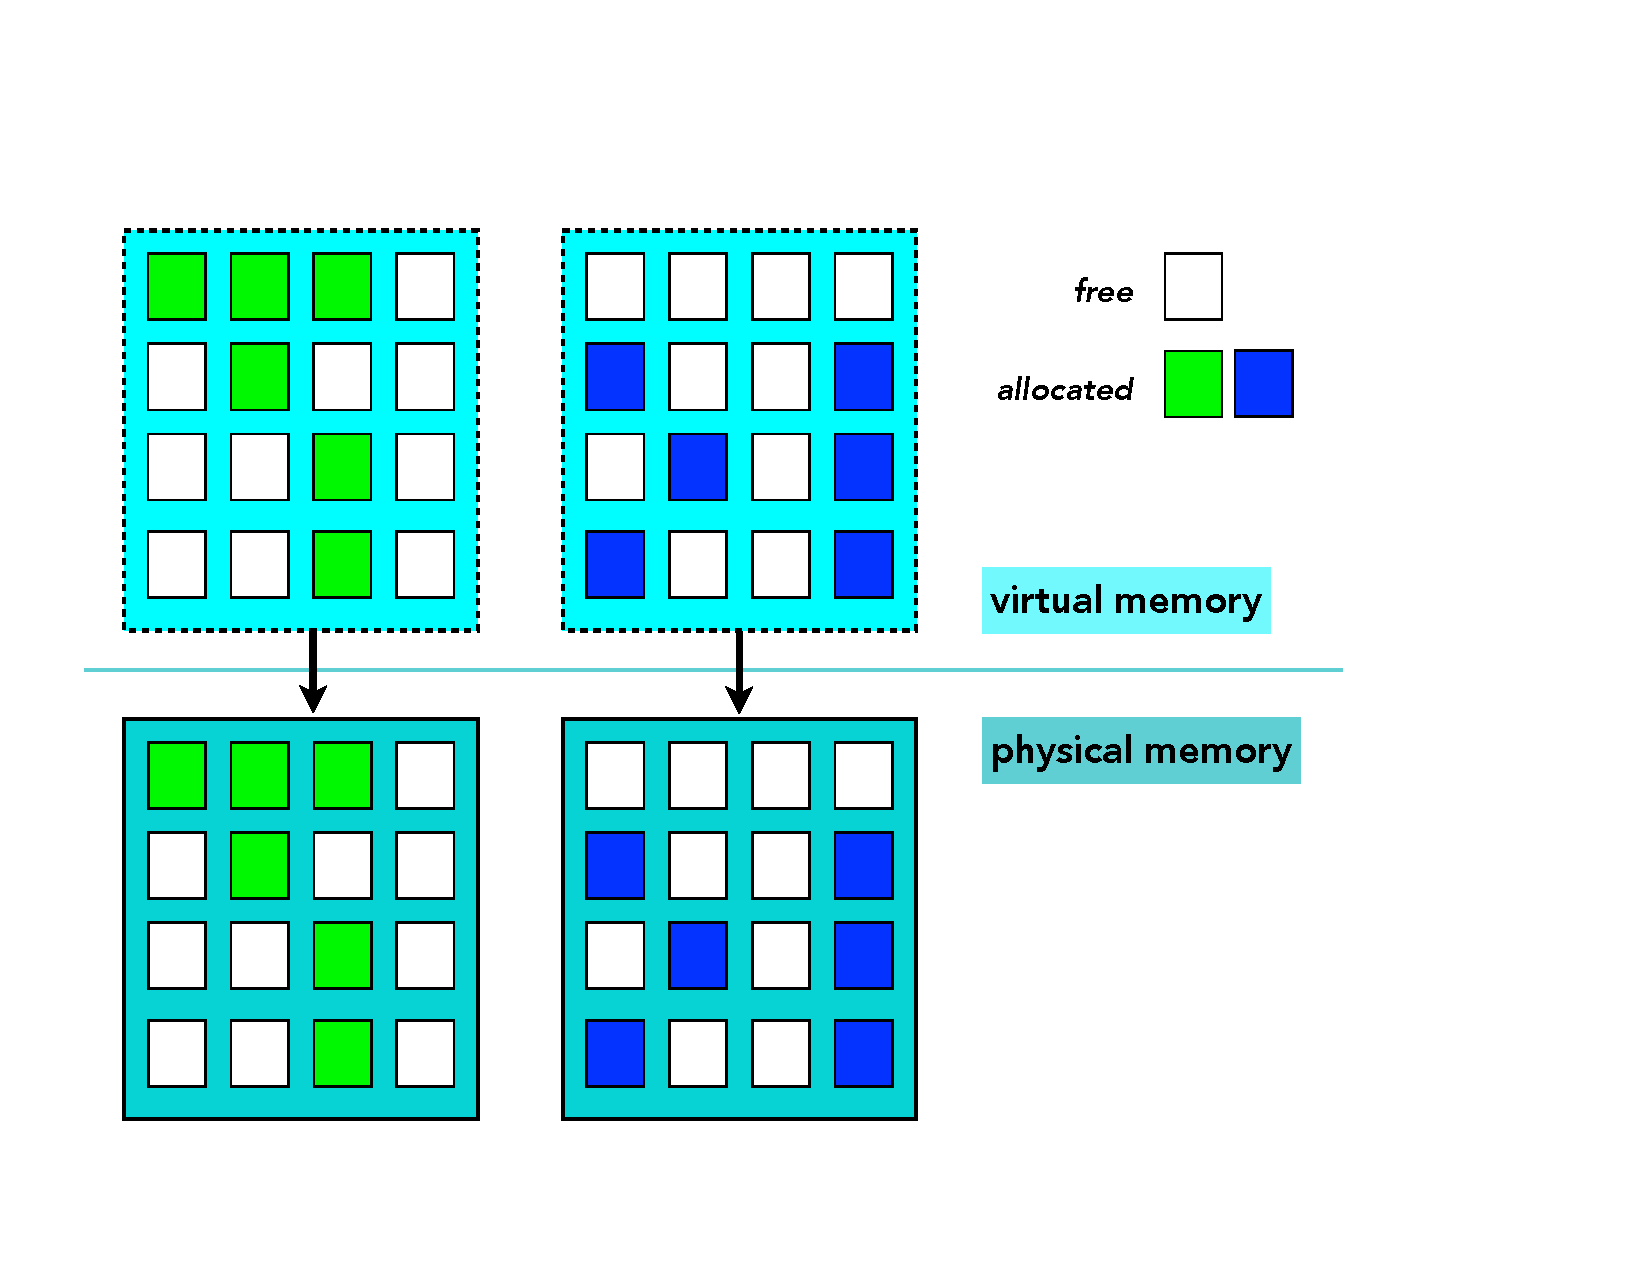
\includegraphics[width=0.45\textwidth]{Chapters/mesh/figures/mesh-diagram-1}
      \label{pre-meshing}
  }
  ~~~~~
  \centering
  \subfloat[\textbf{After:} both virtual pages now point to the
      first physical page; the second page is now freed.]{
      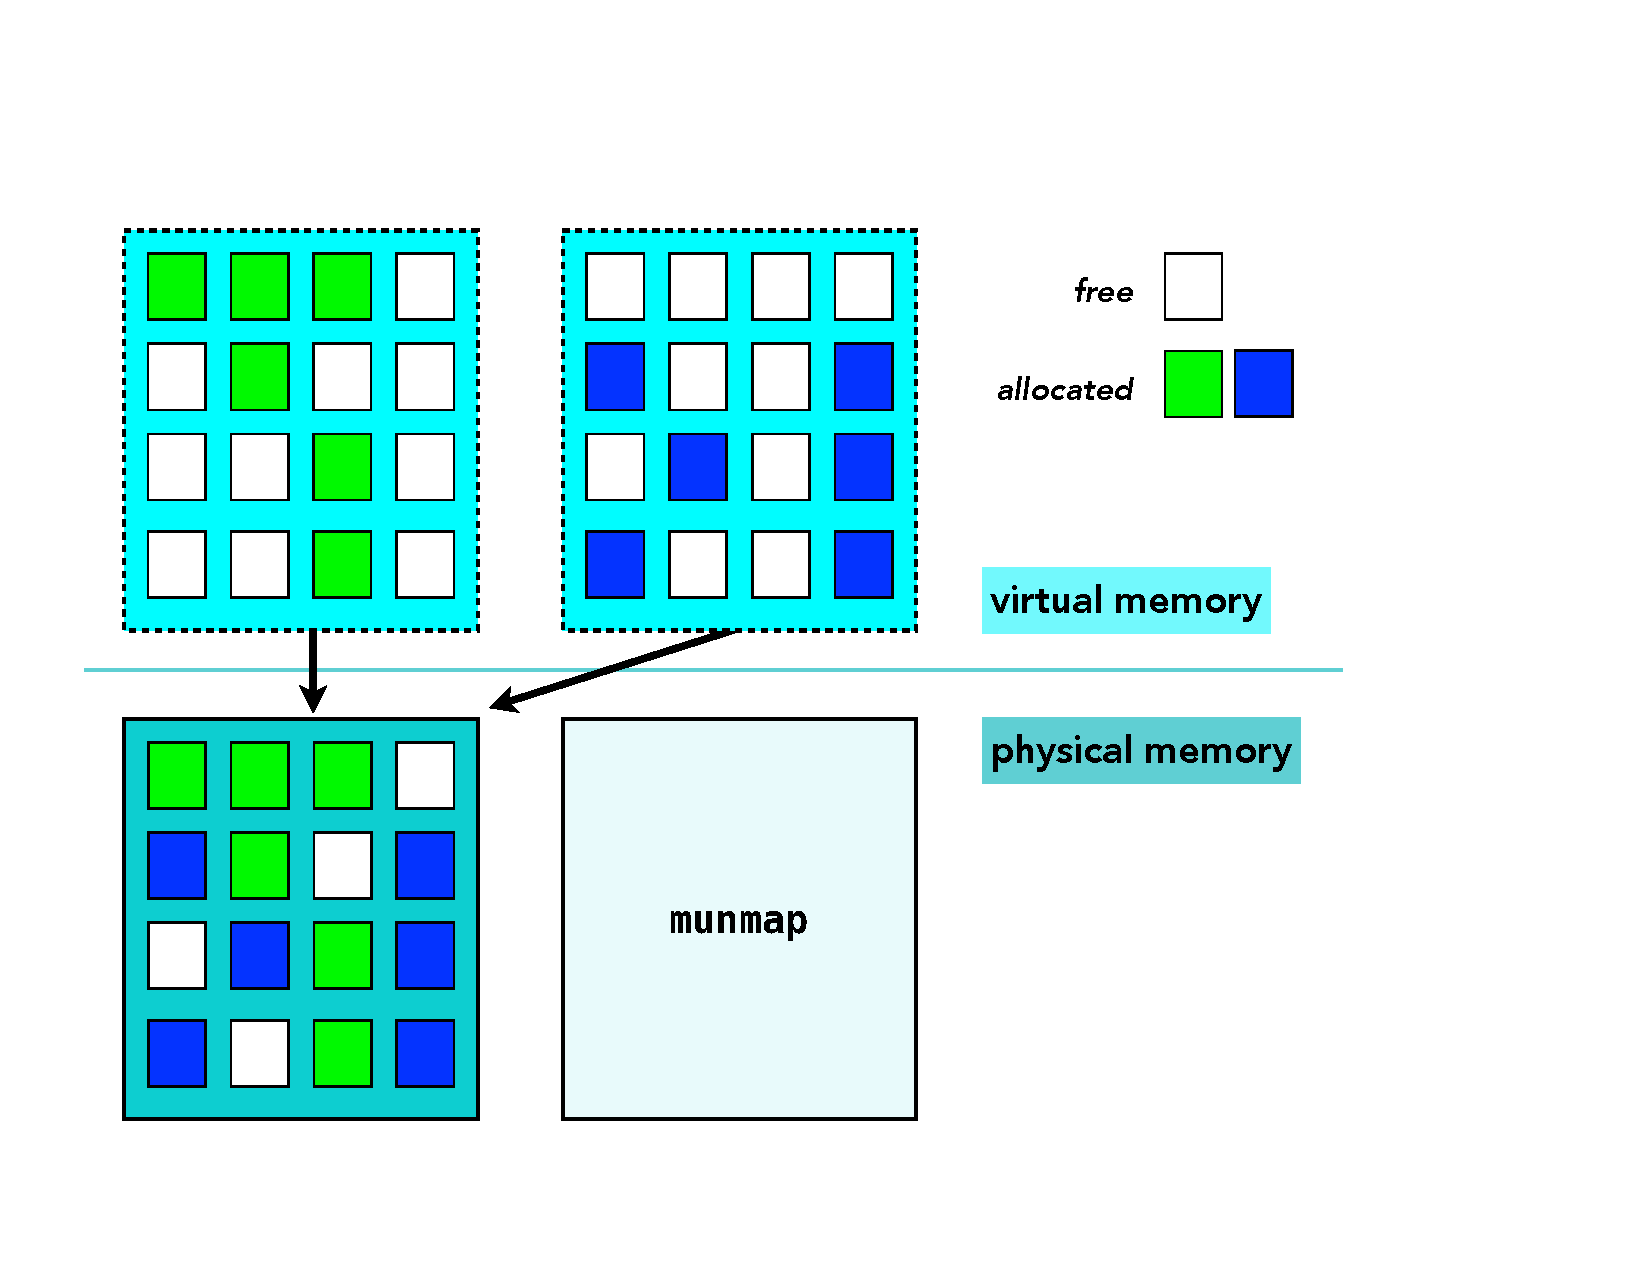
\includegraphics[width=0.45\textwidth]{Chapters/mesh/figures/mesh-diagram-2}
      \label{post-meshing}
  }

  \caption{\textbf{\Mesh{} in action.} \Mesh{} employs novel
    randomized algorithms that let it efficiently find and then
    ``mesh'' candidate pages within \emph{spans} (contiguous 4K pages)
    whose contents do not overlap.  In this example, it increases
    memory utilization across these pages from 37.5\% to 75\%, and
    returns one physical page to the OS (via \texttt{munmap}),
    reducing the overall memory footprint. \Mesh{}'s randomized
    allocation algorithm ensures meshing's effectiveness with high
    probability.}

  \label{fig:meshing}
\end{figure*}


\iffalse
\begin{figure*}[t!]
  \centering
  {
      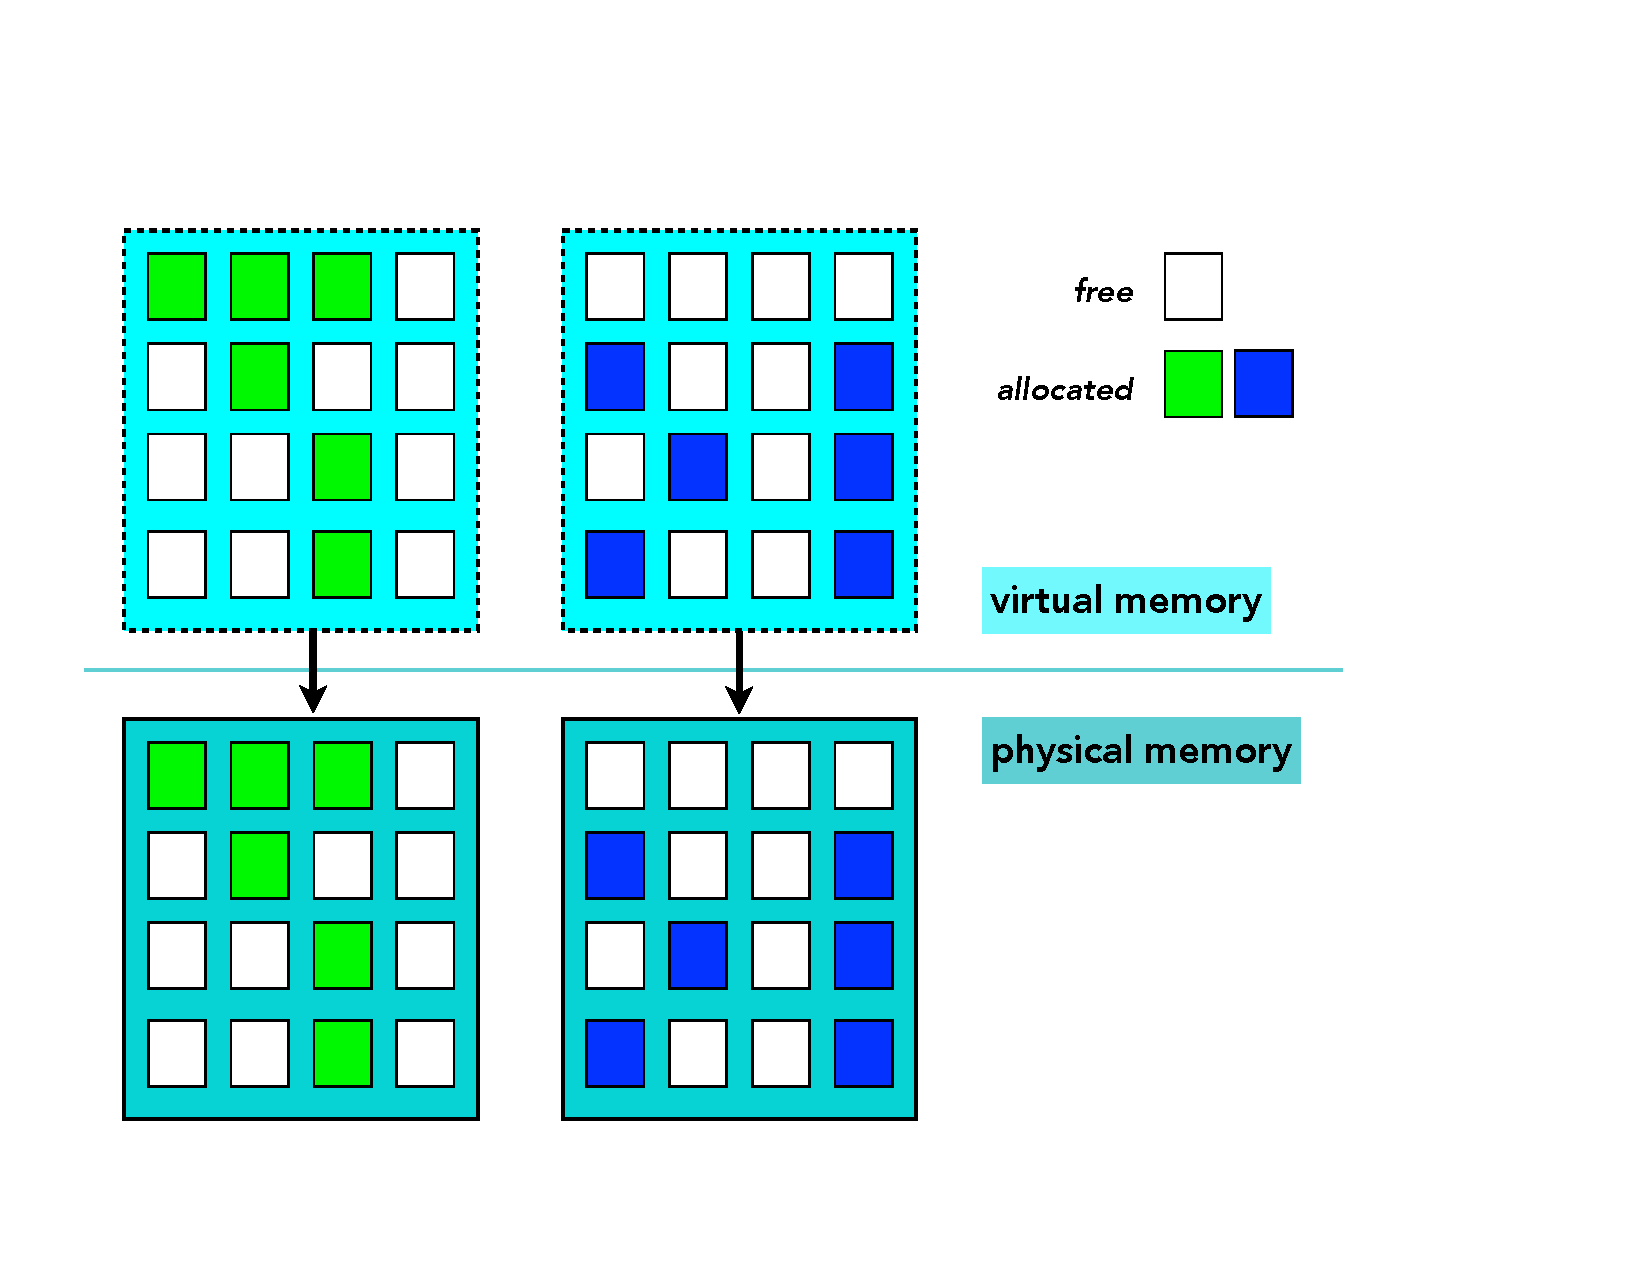
\includegraphics[width=0.45\textwidth]{Chapters/mesh/figures/mesh-diagram-1}
  }

  \caption{\textbf{\Mesh{} in action.} \Mesh{} employs novel
    randomized algorithms that let it efficiently find and then
    ``mesh'' candidate pages within \emph{spans} (contiguous 4K pages)
    whose contents do not overlap.  In this example, it increases
    memory utilization across these pages from 37.5\% to 75\%, and
    returns one physical page to the OS (via \texttt{munmap}),
    reducing the overall memory footprint. \Mesh{}'s randomized
    allocation algorithm ensures meshing's effectiveness with high
    probability.}

  \label{fig:meshing}
\end{figure*}
\fi

\section{Introduction}
\label{sec:introduction}

Memory consumption is a serious concern across the spectrum of modern
computing platforms, from mobile to desktop to datacenters. For
example, on low-end Android devices, Google reports that more than 99
percent of Chrome crashes are due to running out of memory when
attempting to display a web page~\cite{hara:stateofblink}. On
desktops, the Firefox web browser has been the subject of a five-year
effort to reduce its memory footprint~\cite{awsy}. In datacenters,
developers implement a range of techniques from custom allocators to
other \emph{ad hoc} approaches in an effort to increase memory
utilization~\cite{jemalloc:exposehints,redis:announcement}.
%% while
%% Google reports that 10\% of CPU cycles in their clusters are spent on
%% memory allocation~\cite{kanev:2015:warehouse-scale}.

A key challenge is that, unlike in garbage-collected environments,
automatically reducing a C/C++ application's memory footprint
via compaction is not possible. Because the addresses of allocated
objects are directly exposed to programmers, C/C++ applications can
freely modify or hide addresses.  For example, a program may stash
addresses in integers, store flags in the low bits of aligned
addresses, perform arithmetic on addresses and later reference them,
or even store addresses to disk and later reload them.  This hostile
environment makes it impossible to safely relocate objects: if an
object is relocated, all pointers to its original location must be
updated. However, there is no way to safely update \emph{every}
reference when they are ambiguous, much less when they are absent.

Existing memory allocators for C/C++ employ a variety of
best-effort heuristics aimed at reducing average
fragmentation~\cite{johnstone:1998:fragmentation}. However, these
approaches are inherently limited. In a classic result, Robson showed
that all such allocators can suffer from catastrophic
memory fragmentation~\cite{robson:1977:worstcasefrag}. This increase
in memory consumption can be as high as the $\log$ of the ratio
between the largest and smallest object sizes allocated. For example,
for an application that allocates 16-byte and 128KB objects, it is
possible for it to consume $13\times$ more memory than required.

%Embedded systems designed for the Internet-of-Things (IoT), such as the Raspberry Pi Zero W, ship with wireless networking, 3D graphics, and complete operating system stacks but only hundreds of megabytes of memory~\cite{rpi:zero}, placing memory at a premium.

%% TODO: talk about / cite Detlefs paper on precise GC for C/C++

%% address manipulations.  XOR encoding of linked lists

% These addresses can then be freely manipulated: it is legal for C and C++ programs to

% Here, we define fragmentation as the
%amount of memory actually consumed divided by the amount of memory
%actually needed (the total live size).

\begin{comment}
  The result is that C and C++ programs can suffer from fragmentation
(both internal and external). In a setting where compaction
is possible, fragmentation can always be eliminated by squeezing out
space between objects. Since relocating objects is impossible,
fragmentation in C and C++ can become problematic.
\end{comment}

\begin{comment}
  % Push to related work
In languages like LISP, Java and
~\cite{hansen:1969:compaction,fenichel:1969:compaction}, the runtime
system can, as part of garbage collection, periodically compact memory
by moving live objects together. Compaction reduces the working set of
an application and can ensure that an application's footprint never
exceeds some pre-established maximum. Contemporary runtimes like the
Hotspot JVM~\cite{microystems2006memory}, the .NET
VM~\cite{microsoft:dotnet-gc}, and the SpiderMonkey JavaScript
VM~\cite{mozilla:spidermonkey-compaction} implement compaction as part
of their garbage collection algorithms.
\end{comment}


% additionally: build invalid addresses but never dereference them

% emacs pickle state?

%For example, on modern
%systems with a 4 KiB page size and a 16-byte minimum object size, this
%factor corresponds to a worst-case fragmentation of approximately
%$7\times$. In practice, of course, fragmentation is rarely so extreme,
%b
%% TODO: Memory remains one of the scarcest resources across the spectrum of modern computing devices, ranging from servers to desktops to mobile platforms.

%% Not sure - For example, Google reports that \emph{99 percent} of Chrome crashes on low-end Android devices are caused by it running out of memory when attempting to display the page~\cite{hara:stateofblink}.

%% TODO: cost of memory on Amazon servers!

Despite nearly fifty years of conventional wisdom indicating that
compaction is impossible in unmanaged languages, this paper shows that
it is not only possible but also practical. It introduces
\Mesh, a memory allocator that effectively and efficiently performs
compacting memory management to reduce memory usage in unmodified
C and C++ applications.

Crucially and counterintuitively, \Mesh performs compaction without
relocation; that is, without changing the addresses of objects. This
property is vital for compatibility with arbitrary C/C++
applications. To achieve this, \Mesh{} builds on a mechanism which we
call \emph{meshing}, first introduced by Novark et al.'s Hound memory
leak detector~\cite{1542521}. Hound employed meshing in an effort to avoid
catastrophic memory consumption induced by its memory-inefficient
allocation scheme, which can only reclaim memory when every object on
a page is freed. Hound first searches for pages whose live objects do
not overlap. It then copies the contents of one page onto the other,
remaps one of the \emph{virtual} pages to point to the single
\emph{physical} page now holding the contents of both pages, and
finally relinquishes the other physical page to the
OS. Figure~\ref{fig:meshing} illustrates meshing in action.

\Mesh{} overcomes two key technical challenges of meshing that previously made
it both inefficient and potentially entirely ineffective. First,
Hound's search for pages to mesh involves a linear scan of pages on
calls to \texttt{free}. While this search is more efficient than a
naive $O(n^2)$ search of all possible pairs of pages, it remains
prohibitively expensive for use in the context of a general-purpose
allocator. Second, Hound offers no guarantees that \emph{any} pages
would ever be meshable.  Consider an application that happens to
allocate even one object in the same offset in every page. That layout
would preclude meshing altogether, eliminating the possibility of
saving any space.

\Mesh makes meshing both efficient and provably effective (with high
probability) by combining it with two novel randomized
algorithms. First, \Mesh uses a space-efficient randomized
allocation strategy that effectively scatters objects within each
virtual page, making the above scenario provably exceedingly
unlikely. Second, \Mesh incorporates an efficient randomized
algorithm that is guaranteed with high probability to quickly find
candidate pages that are likely to mesh. These two algorithms work in
concert to enable formal guarantees on \Mesh's effectiveness. Our
analysis shows that \Mesh breaks the above-mentioned Robson worst
case bounds for fragmentation with high
probability~\cite{robson:1977:worstcasefrag}, as memory reclaimed by meshing is available for use by any size class.
This ability to redistribute memory from one size class to another enables Mesh to adapt to changes in an application's allocation behavior in a way other segregated-fit allocators cannot.


We implement \Mesh as a library for C/C++ applications running on
Linux or Mac OS X. \Mesh{} interposes on memory management operations,
making it possible to use it without code changes or
recompilation by setting the appropriate environment variable to load
the \Mesh{} library (e.g., \texttt{export
  LD\_PRELOAD=libmesh.so} on Linux). Our evaluation demonstrates that
our implementation of \Mesh{} is both fast and efficient in
practice. It generally matches the performance of state-of-the-art
allocators while guaranteeing the absence of catastrophic
fragmentation with high probability. In addition, it occasionally
yields substantial space savings: replacing the standard allocator
with \Mesh{} automatically reduces memory consumption by 16\%
(Firefox) to 39\% (Redis).
%In
%general, the longer-lived and more memory-intensive the application,
%the more memory \Mesh can save.


\subsection{Contributions}
\label{sec:contributions}

This paper makes the following contributions:

\begin{itemize}

\item It introduces \textbf{\Mesh}, a novel memory allocator that acts
  as a plug-in replacement for \texttt{malloc}. \Mesh{} combines
  remapping of virtual to physical pages (meshing) with randomized
  allocation and search algorithms to enable safe and effective
  \emph{compaction without relocation} for C/C++
  (\S\ref{sec:meshing}, \S\ref{sec:algorithms},
  \S\ref{sec:allocator}).

\item It presents theoretical results that guarantee \Mesh{}'s
    efficiency and effectiveness with high probability (\S\ref{sec:theory}).

\item It evaluates \Mesh{}'s performance empirically, demonstrating \Mesh{}'s ability to reduce
    space consumption while generally imposing low runtime
    overhead (\S\ref{sec:evaluation}).

\end{itemize}


\section{Overview}
\label{sec:meshing}

\begin{comment}
  \begin{figure}[!t]
\centering
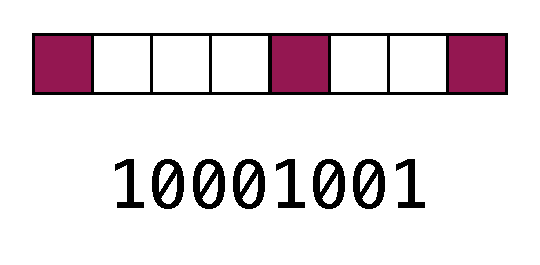
\includegraphics[width=.3\textwidth]{figures/bitmap_bitstring}
\caption{The bitmaps managing the allocated space in a span
  (visualized as allocated objects in the span, top) can be
  represented as bitstrings of 0s and 1s (bottom), where a 1
  corresponds to an allocated object and 0 to free space.}
\label{fig:bitmap-bitstring}
\end{figure}
\end{comment}

This section provides a high-level overview of how \Mesh{} works and
gives some intuition as to how its algorithms and implementation
ensure its efficiency and effectiveness, before diving into detailed
description of \Mesh{}'s algorithms (\S\ref{sec:algorithms}),
implementation (\S\ref{sec:allocator}), and its theoretical analysis
(\S\ref{sec:theory}).


\subsection{Remapping Virtual Pages}

\Mesh{} enables compaction without relocating object addresses; it
depends only on hardware-level virtual memory support, which is
standard on most computing platforms like x86 and ARM64. \Mesh{} works
by finding pairs of pages and merging them together \emph{physically}
but not \emph{virtually}: this merging lets it relinquish
physical pages to the OS.

Meshing is only possible when no objects on the pages occupy the same
offsets.  A key observation is that as fragmentation increases (that
is, as there are more free objects), the likelihood of successfully
finding pairs of pages that mesh also increases.

Figure~\ref{fig:meshing} schematically illustrates the meshing
process. \Mesh{} manages memory at the granularity of \textit{spans},
which are runs of contiguous 4K pages (for purposes of illustration,
the figure shows single-page spans). Each span only contains
same-sized objects. The figure shows two spans of memory with low
utilization (each is under $40\%$ occupied) and whose allocations are at non-overlapping offsets.


\begin{comment}

More formally, we can say that $t$ spans
\textit{\mesh} if and only if the sum of each offset across the $t$
spans sum to 1 or less:

\begin{align}
  \forall k \in [0, b-1]. \sum_{0 \leq i \leq t} s_i[k] \leq 1
\end{align}

where $b$ is span length, and $s_i[k] = 1$ iff there is an object at the $k$th offset of span i.
\end{comment}

Meshing consolidates allocations from each span onto one physical span.
Each object in the resulting meshed span resides at the same offset as
it did in its original span; that is, its virtual addresses are
preserved, making meshing invisible to the application. Meshing then
updates the virtual-to-physical mapping (the page tables) for the
process so that both virtual spans point to the same physical
span. The second physical span is returned to the OS.  When average
occupancy is low, meshing can consolidate many pages, offering the
potential for considerable space savings.
% consolidated to a single span and all other spans can be reused.


\subsection{Random Allocation}

A key threat to meshing is that pages could contain objects at the
same offset, preventing them from being meshed. In the worst case, all
spans would have only one allocated object, each at the same offset,
making them non-meshable. \Mesh{} employs randomized allocation to
make this worst-case behavior exceedingly unlikely. It allocates
objects uniformly at random across all available offsets in a span. As
a result, the probability that all objects will occupy the same offset
is $\left({1}/{b}\right)^{n-1}$, where $b$ is the number of objects in
a span, and $n$ is the number of spans.

%Meshing employs random allocation to minimize the likelihood of this happening too often. The use of a randomized algorithm lets us reason about the effectiveness of meshing in expectation.

%Meshing introduces a limited amount of randomness to ensure that we
%can reason about meshing spans in expectation.

In practice, the resulting probability of being unable to mesh many
pages is vanishingly small. For example, when meshing 64 spans with
one 16-byte object allocated on each (so that the number of objects
$b$ in a 4K span is $256$), the likelihood of being unable to mesh any
of these spans is $10^{-152}$. To put this into perspective, there are
estimated to be roughly $10^{82}$ particles in the universe.

We use randomness to guide the design of \Mesh{}'s algorithms
(\S\ref{sec:algorithms}) and implementation (\S\ref{sec:allocator});
this randomization lets us prove robust guarantees of its performance
(\S\ref{sec:theory}), showing that \Mesh{} breaks the Robson bounds with
high probability.

% ,
%subject to an assumption that application allocation behavior does not
%depend on the addresses returned by the allocator.

%% TODO: should insert a treatment of Emery's ideas about address obliviousness somewhere.


\subsection{Finding Spans to Mesh}

Given a set of spans, our goal is to mesh them in a way that frees as
many physical pages as possible. We can think of this task as that of
partitioning the spans into subsets such that the spans in each subset
mesh. An optimal partition would minimize the number of such subsets.

%% TODO: fix ref to point at exact subsection in algorithms.

Unfortunately, as we show, optimal meshing is not feasible
(\S\ref{sec:theory}). Instead, the algorithms in
Section~\ref{sec:algorithms} present practical methods for finding
high-quality meshes under real-world time constraints. We show that
solving a simplified version of the problem (\S\ref{sec:algorithms})
is sufficient to achieve reasonable meshes with high probability
(\S\ref{sec:theory}).


\begin{comment}
Memory fragmentation, introduced in Section~\ref{sec:introduction},
occurs when the ratio of program-allocated memory to operating-system
reserved memory becomes high:

\begin{align*}
\text{Fragmentation} = \frac{\text{Reserved}}{\text{Allocated}}
\end{align*}

\end{comment}

%%\textit{XXX: I think it is worth noting that an allocator that stored a very high amount of metadata per allocation (e.g. tracking the   meshability graph explicitly) would be indistinguishable from a   highly-fragmented allocator from the perspective of the OS.  Not   sure how to work that in.}

%% Informally, fragmentation occurs because the application manages
%% memory in bytes, while the operating system manages memory at page
%% granularity -- 4 KiB on most current architectures.  Sparsely allocated
%% application addresses ``pin down'' otherwise vacant OS pages.

%% Many managed languages like Java and JavaScript do not experience
%% memory fragmentation due to the combination of language soundness and
%% garbage collection implementations.  Languages are designed in such a
%% way that implementations can enumerate and update all object
%% references, enabling garbage collectors to periodically compact live
%% objects.  This isn't possible for unmanaged languages like C, C++ and
%% Rust, as it is not possible to soundly enumerate all object
%% references.


%% XXX: we should unify talking about ``objects'' and ``allocations''
%% -- allocations is probably better for unmanaged languages where
%% objects have a specific interpretation.

%% Meshing works on \textit{spans} -- contiguous regions of memory where
%% the size of a span is a multiple of the page size between 4 KiB and
%% 128 KiB.  Each span allocates objects of a single-size only, for
%% example a 4 KiB span might hold 32 objects of size 128 bytes.  We can
%% represent a span by a \textit{bitstring}, as in
%% Figure~\ref{fig:bitmap-bitstring}, a string with a 1 for an allocated
%% object at that offset from the start of the span and 0 otherwise.  The
%% length of the bitstring is the number of objects that span holds.

%% This definition characterizes the constraints of the technique by
%% which meshing is possible, wherein two or more spans are meshed or
%% "stacked" on top of each other.

%% The layout and management of a program's heap guide how we consider
%% meshing.  In a running program, the heap is managed as a number of
%% different \textit{size classes} along with a region consisting of
%% large allocations.  Allocations are fulfilled from the smallest size
%% class they fit in (e.g. an allocation request for 50 bytes is
%% satisfied by the 64-byte size class), and objects larger than 16 KiB
%% are individually served from the large allocation region.

%% We treat each size class as an independent instance of the meshing
%% problem, and large allocations are not meshed.  As large allocations
%% are all many multiples of the page size significant fragmentation
%% between them does not exist.  The number of size-classes is fixed at
%% compilation time and constant during the execution of a program.

%% From here, we consider meshing as dealing with a single size-class,
%% and refer to all spans within this size class as $S$.  If we want to
%% mesh the entire heap, this means solving $n$ instances of the meshing
%% problem, where $n$ is the number of size classes.


%% Finally, meshing relies on the fact that there are two types of spans,
%% virtual and physical.  A \textit{virtual} span refers to the memory
%% addresses visible to the program being executed, while a
%% \textit{physical} span corresponds to the area in memory where
%% allocated objects live.  Meshing is concerned with minimizing the
%% count of in-use physical spans without modifying or moving virtual
%% spans.  As noted in Section~\ref{sec:introduction}, we cannot change
%% or modify virtual addresses returned from the allocator, as we do not
%% have a way to enumerate and update all references the program has
%% stored.  Since the last two digits of a virtual address directly
%% specify the offset of the referenced object in the span, objects
%% cannot be safely relocated to a different offset, leading to our

%% Allocated objects and free space within a span are tracked by the
%% memory allocator as a bitmap (see Section~\ref{sec:allocator}) -- the
%% in-memory representation of a bitstring.  For example, for objects of
%% size 32 and a span size of 4 KiB, the span can hold 128 32-byte
%% objects, so allocated objects are be tracked with a 128-bit bitmap.
%% Each allocated object in a running program has a unique
%% \textit{(bitmap, offset)} tuple.  Bitmaps are between 8 and 256-bits
%% in length.

%% We can therefore think of the meshing problem as that of partitioning
%% a set of equal-length bitstrings such that the bitstrings in each subset
%% mesh.  An optimal partition would minimize the number of such subsets.
%% This abstraction allows us to analyze the complexity of this computational
%% task in Section~\ref{sec:theory}.


\section{Algorithms \& System Design}
\label{sec:algorithms}

%This section provides an overview of \Mesh{}'s algorithms.
%Section~\ref{sec:allocator} provides a detailed description of \Mesh's
%implementation, while Section~\ref{sec:theory} presents a theoretical
%analysis of its effectiveness.

\Mesh{} comprises three main algorithmic components: allocation
(\S\ref{sec:allocation-algorithm}), deallocation
(\S\ref{sec:deallocation-algorithm}), and finding spans to mesh
(\S\ref{sec:meshing-algorithm}). Unless otherwise noted and without
loss of generality, all algorithms described here are per size class
(within spans, all objects are same size).

\subsection{Allocation}
\label{sec:allocation-algorithm}
% We want out allocator to enforce random spread of objects so that we can probabilistically guarantee meshing.  Also we want it to reuse memory when available.

Allocation in \Mesh{} consists of two steps: (1) finding a span to
allocate from, and (2) randomly allocating an object from that span.
\Mesh{} always allocates from a thread-local shuffle vector -- a
randomized version of a freelist %(described in detail in\S\ref{sec:shuffle-freelists}). 
The shuffle vector contains offsets
corresponding to the slots of a single span.  We call that span the
\emph{attached} span for a given thread.

If the shuffle vector is empty, \Mesh relinquishes the current
thread's attached span (if one exists) to the \emph{global heap}
(which holds all unattached spans), and asks it to select a new
span. If there are no partially full spans, the global heap returns a
new, empty span.  Otherwise, it selects a partially full span for
reuse. To maximize utilization, the global heap groups spans into bins
organized by decreasing occupancy (e.g., 75-99\% full in one bin,
50-74\% in the next). The global heap scans for the first non-empty
bin (by decreasing occupancy), and randomly selects a span from that
bin.

Once a span has been selected, the allocator adds the offsets
corresponding to the free slots in that span to the thread-local
shuffle vector (in a random order). \Mesh{} pops the first entry off
the shuffle vector and returns it.


\subsection{Deallocation}
\label{sec:deallocation-algorithm}

Deallocation behaves differently depending on whether the free is
local (the address belongs to the current thread's attached span),
remote (the object belongs to another thread's attached span), or if
it belongs to the global heap.

For local frees, \Mesh{} adds the object's offset onto the span's
shuffle vector in a random position and returns. For remote frees,
\Mesh{} atomically resets the bit in the corresponding index in a
bitmap associated with each span. Finally, for an object belonging to
the global heap, \Mesh{} marks the object as free, updates the span's
occupancy bin; this action may additionally trigger meshing.
%, which we
%describe below.

%% Global frees similarly mark the space backing an allocation as free and open for reuse in the owning span, but additionally may trigger meshing.  Meshing happens after a global free if it has been more than a set period of time since the last meshing (settable both at program startup and later by the program through the \texttt{mallctl} API, by default a tenth of a second, and if the allocator thinks there is a reasonable chance of meshing reclaiming space.

%% TODO: free -- right now, we assume unlimited virtual addresses; max limit of ranges in kernel (discuss in implementation)


\subsection{Meshing}
\label{sec:meshing-algorithm}

When meshing, \Mesh{} randomly chooses pairs of spans and attempts to
mesh each pair. The meshing algorithm, which we call \sm
(Figure~\ref{fig:meshalg}), is designed both for practical
effectiveness and for its theoretical guarantees.  The parameter $t$,
which determines the maximum number of times each span is probed (line
\ref{li:outerloop}), enables space-time trade-offs. The parameter $t$
can be increased to improve mesh quality and therefore reduce space,
or decreased to improve runtime, at the cost of sacrificed meshing
opportunities. We empirically found that $t=64$ balances runtime and
meshing effectiveness, and use this value in our implementation.

\sm proceeds by iterating through $S_l$ and checking whether it can
mesh each span with another span chosen from $S_r$ (line
\ref{li:condition}).  If so, it removes these spans from their
respective lists and meshes them (lines
\ref{li:remove}--\ref{li:mesh}). \sm repeats until it has checked $t *
|S_l|$ pairs of spans; \S\ref{sec:meshing-implementation} describes
the implementation of \sm in detail.

\begin{comment}
  At this point, each span has been checked exactly once.  All spans not
removed from the lists are still candidates for meshing.  \sm loops
again through the lists, in the $j$th step comparing the $j$th span in
$S_l$ with the $j+1$th span in $S_r$.  Again, whenever it compares a
pair of spans that can mesh, it removes them from their respective
lists and meshes them.

\sm repeats this looping process $t$ times.  On the $i$th loop through
the lists, the $j$th element in $S_l$ is compared with the $j+i-1$th
element in $S_r$.  After this outer loop (line~\ref{li:outerloop}) has
completed, any remaining span has been compared with $t$ other spans,
each time failing to mesh. \sm stops here and makes no further effort
to mesh these spans.
\end{comment}


\iffalse
\begin{algorithm}[tb]
  \LinesNumbered
  \SetKwData{Frontier}{frontier}\SetKwData{This}{this}\SetKwData{OldNode}{$n_{old}$}\SetKwData{NewNode}{$n_{new}$}
  \SetKw{Continue}{continue} \SetKw{And}{and}
  \SetKwData{Null}{null}
  \SetKwData{Path}{path}
  \SetKwData{OldEdges}{$E_{old}$}
  \SetKwData{NewEdges}{$E_{new}$}
  \SetKwData{OldEdge}{$e_{old}$}
  \SetKwData{NewEdge}{$e_{new}$}
  \SetKwData{Length}{Length}
  \SetKwData{True}{true} \SetKwData{False}{false}
  \SetKwFunction{MakeTuple}{MakeTuple}
  \SetKwFunction{GetRoot}{GetRoot}\SetKwFunction{Enqueue}{enqueue}\SetKwFunction{Length}{length}\SetKwFunction{Dequeue}{dequeue}
  \SetKwFunction{HasVisited}{HasVisited}
  \SetKwFunction{MarkAsVisited}{MarkAsVisited}
  \SetKwFunction{MarkAsGrowing}{MarkAsGrowing}
  \SetKwFunction{MarkNotGrowing}{MarkNotGrowing}
  \SetKwFunction{RecordGrowingPath}{RecordGrowingPath}
  \SetKwFunction{IsGrowing}{IsGrowing}
  \SetKwInOut{Input}{Input}\SetKwInOut{Output}{Output}
  \Input{$G_{final} = (N, E)$}
  \Frontier$\leftarrow$ []\;
  $n_{root} \leftarrow$ \GetRoot{$G_{final}$}\;
  \For{$e = (n_1, n2) \in E : n_1 = n_{root}$}{
    \Frontier.\Enqueue{\MakeTuple{\Null, $e$}}
  }
  \While{\Frontier.\Length $\neq 0$}{
    $T \leftarrow$ \Frontier.\Dequeue{}\;
    $(T_{prev}, e) \leftarrow T$\;
    \eIf{\HasVisited{$e$}}{
      \Continue\;
    }{
      \MarkAsVisited{$e$}\;
    }
    $(n_{from}, n_{to}) \leftarrow e$\;

    \If{\IsGrowing{$n_{to}$}}{
      \RecordGrowingPath{$T$}\;
    }
    \ForEach{$e=(n_1,n_2) \in E : n_1 = n_{to}$}{
      \Frontier.\Enqueue{\MakeTuple{$T$, $e$}}\;
    }
  }
  \caption{FindLeakPaths, which records paths through the heap to leaking nodes. RecordGrowingPath recovers the entire path to the edge $e$ by following the linked list formed by the tuple $T$.}
  \label{algo:findpaths}
\end{algorithm}
\fi

\iffalse
\begin{algorithm}[tb]
  \SetAlgorithmName{\sm}{}{}
  \SetKwInOut{Input}{Input}
  \SetKwInOut{Output}{Output}
  \Input{randomly ordered list of spans S, $|S| = n$; parameter $t$}

  M $ \leftarrow$ []\;

  $S_l,$ $S_r = S[1:\frac{n}{2}],$ $S[\frac{n}{2}+1 : n]$\;
  \ForEach{$i \in [0, t-1]$}{
    len = length$(S_l)$\;
    \ForEach{$j \in [0, \frac{n}{2}-1]$}{
      \If{$S_l(j)$ and $S_r(j+i$ mod len) mesh}{
        $S_l \leftarrow S_l \textbackslash S_l(j)$\;
        $S_r \leftarrow S_r \textbackslash S_r(j+i$ mod len)\;
        M $\leftarrow$ M $\cup$ $S_l(j)$ $\cup$ $S_r(j+i$ mod len)\;
      }
    }
  }
  \Return M\;
  \TitleOfAlgo{Procedure splits span set into halves and probes for meshable pairs between halves.}
%  \label{alg:mesher}
\end{algorithm}
\fi

\begin{figure}[!t]
\begin{codebox}
    \Procname{$\sm(S,t)$}
%    \li M $\gets$ []
    \li $n \gets$ length$(S)$
    \li $S_l,$ $S_r \gets S[1:n/2],$ $S[n/2 +1 : n]$
    \li \For $(i = 0, i<t, i++)$ \label{li:outerloop}
        \li \Do
            $\mbox{len} = |S_l|$\;
            \li \For $(j = 0, j < \mbox{len}, j++)$ \label{li:innerloop}
                \li \Do
                    \If \proc{Meshable} $(S_l(j)$, $S_r(j+i$ \% $\mbox{len}$)) \Then \label{li:condition}
                        \li $S_l \leftarrow S_l \setminus S_l(j)$ \label{li:remove}
                        \li $S_r \leftarrow S_r \setminus S_r(j+i$ \% $\mbox{len}$)
%                        \li M $\leftarrow$ M $\cup$ $S_l(j)$ $\cup$ $S_r(j+i$ mod len)
                        \li \proc{mesh}($ S_l(j)$, $S_r(j+i$ \% $\mbox{len}$)) \label{li:mesh}
                    \End
                \End
        \End
%    \li \Return M
\end{codebox}
\caption{\textbf{Meshing random pairs of spans.} \sm splits the randomly ordered span list $S$ into halves, then probes pairs between halves for meshes.  Each span is probed up to $t$ times.}
\label{fig:meshalg}
\end{figure}


\section{Implementation}
\label{sec:allocator}

We implement \Mesh as a drop-in replacement memory allocator that
implements meshing for single or multi-threaded applications written
in C/C++. Its current implementation work for 64-bit Linux and Mac OS
X binaries. \Mesh can be explicitly linked against by passing
\texttt{-lmesh} to the linker at compile time, or loaded dynamically
by setting the \texttt{LD\_PRELOAD} (Linux) or
\texttt{DYLD\_INSERT\_LIBRARIES} (Mac OS X) environment variables to
point to the \Mesh{} library. When loaded, \Mesh interposes on
standard libc functions to replace all memory allocation functions.

\begin{comment}
\begin{figure}
  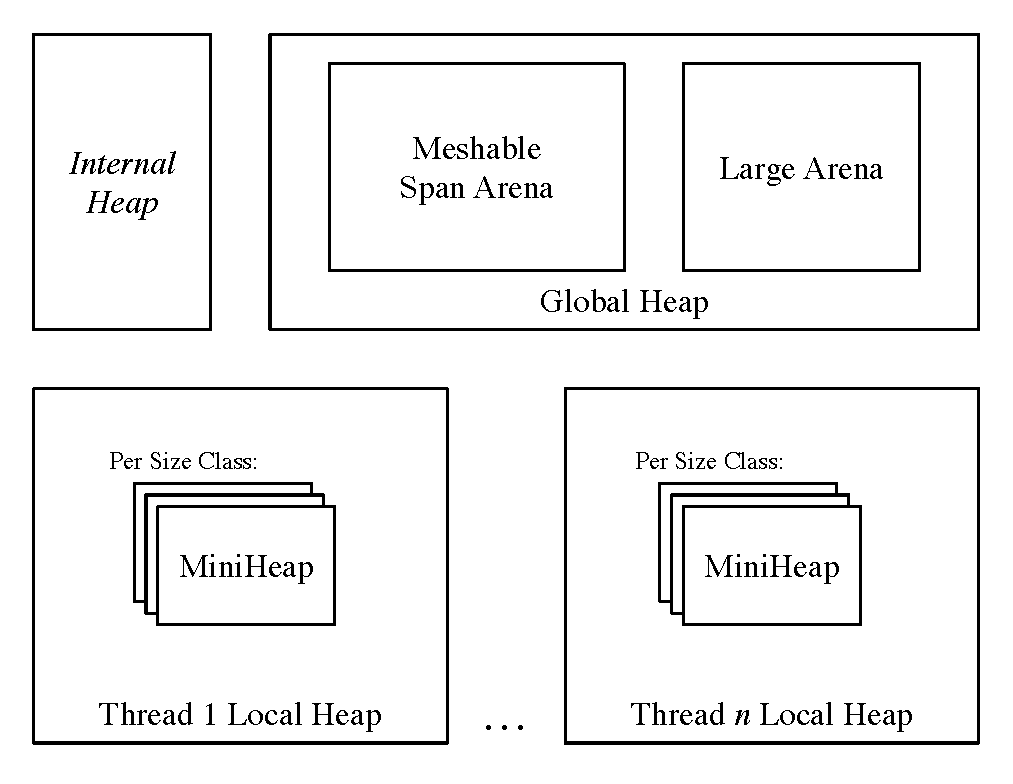
\includegraphics[width=.5\textwidth]{figures/global_heap}
  \caption{\textbf{Heap organization.} \Mesh's internal allocator
    manages memory for \Mesh-internal dynamic data structures.
    The global heap manages both large objects and the meshable arena that spans are allocated from.  Each thread has a
    local heap which satisfies small allocations from MiniHeaps (one
    per size class).}
  \label{fig:global-heap}
\end{figure}
\end{comment}

\Mesh combines traditional allocation strategies with meshing to
minimize heap usage.  Like most modern memory
allocators~\cite{Novark:2010:DSH:1866307.1866371,1134000,379232,evans2006scalable,ghemawattcmalloc},
\Mesh is a segregated-fit allocator. \Mesh{} employs fine-grained size
classes to reduce internal fragmentation due to rounding up to the
nearest size class. \Mesh{} uses the same size classes as those
used by jemalloc for objects 1024 bytes and
smaller~\cite{evans2006scalable}, and power-of-two size classes for
objects between 1024 and 16K.  Allocations are fulfilled from the
smallest size class they fit in (e.g., objects of size 33--48 bytes
are served from the 48-byte size class); objects larger than 16K are
individually fulfilled from the global arena.  Small objects are
allocated out of \textit{spans} (\S\ref{sec:meshing}), which are
multiples of the page size and contain between 8 and 256 objects of a
fixed size.  Having at least eight objects per span helps
amortize the cost of reserving memory from the global manager for
the current thread's allocator.

Objects of 4KB and larger are always page-aligned and span at least one
entire page. \Mesh does not consider these objects for meshing;
instead, the pages are directly freed to the OS.

\Mesh's heap organization consists of four main components.
\emph{MiniHeaps} track occupancy and other metadata for spans
(\S\ref{sec:miniheaps}).  \textit{Shuffle vectors} enable efficient,
random allocation out of a MiniHeap (\S\ref{sec:shuffle-freelists}).
\textit{Thread local heaps} satisfy small-object allocation requests
without the need for locks or atomic operations in the common case
(\S\ref{sec:thread-local-heaps}). Finally, the \textit{global heap}
(\S\ref{sec:global-heap}) manages runtime state shared by all threads,
large object allocation, and coordinates meshing operations
(\S\ref{sec:meshing-implementation}).


\subsection{MiniHeaps}
\label{sec:miniheaps}

MiniHeaps manage allocated physical spans of memory and are either
\emph{attached} or \emph{detached}.  An attached MiniHeap is owned by
a specific thread-local heap, while a detached MiniHeap is only
referenced through the global heap.  New small objects are
\textit{only} allocated out of attached MiniHeaps.

Each MiniHeap contains metadata that comprises span length, object
size, allocation bitmap, and the start addresses of any virtual spans
meshed to a unique physical span.  The number of objects that can be
allocated from a MiniHeap bitmap is \textit{objectCount = spanSize /
  objSize}.  The allocation bitmap is initialized to
\textit{objectCount} zero bits.

When a MiniHeap is attached to a
thread-local \emph{shuffle vector} (\S\ref{sec:shuffle-freelists}),
each offset that is unset in the MiniHeap's bitmap is added to the
shuffle vector, with that bit now atomically set to one in the bitmap.
This approach is designed to allow multiple threads to free objects
which keeping most memory allocation operations local in the common
case.

When an object is freed and the free is non-local
(\S\ref{sec:deallocation-algorithm}), the bit is reset.  When a new
MiniHeap is allocated, there is only one virtual span that points to
the physical memory it manages. After meshing, there may be multiple
virtual spans pointing to the MiniHeap's physical memory.


\begin{figure}[!t]
  \centering
  \subfloat[A shuffle vector for a span of size 8, where no objects have
      yet been allocated.]{
      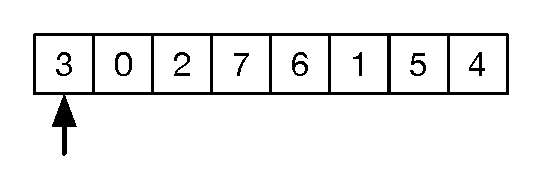
\includegraphics[width=.4\textwidth]{Chapters/mesh/figures/shuffle-freelist_a}
  }
  \vspace{-0em}
  \subfloat[The shuffle vector after the first object has been allocated.]{
      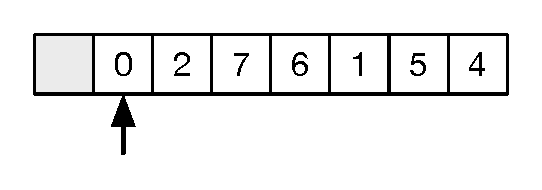
\includegraphics[width=.4\textwidth]{Chapters/mesh/figures/shuffle-freelist_b}
  }
  \vspace{-0em}
  \subfloat[On \texttt{free}, the object's offset is pushed onto the
      front of the vector, the allocation index is updated, and the
      offset is swapped with a randomly chosen offset.]{
      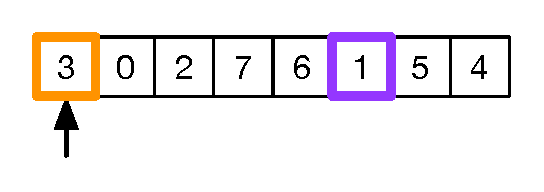
\includegraphics[width=.4\textwidth]{Chapters/mesh/figures/shuffle-freelist_c}
  }
  \vspace{-0em}
  \subfloat[Finally, after the swap, new allocations proceed in a
      bump-pointer like fashion.]{
    \centering
    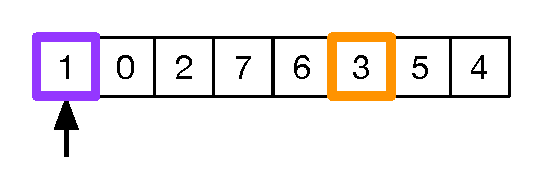
\includegraphics[width=.4\textwidth]{Chapters/mesh/figures/shuffle-freelist_d}
  }
  \vspace{0.5em}
  \caption{\textbf{Shuffle vectors} compactly enable fast random allocation.
    Indices (one byte each) are maintained in random order; allocation is
    popping, and deallocation is pushing plus a random swap (\S\ref{sec:shuffle-freelists}).}
    % When an object is freed and the MiniHeap     it was allocated from is still attached to the local thread,    its
  \label{fig:shuffle-freelists}
\end{figure}


%% TODO: restore locality section if and when we have locality results
\begin{comment}
\subsubsection{Locality}

At first blush, it may appear that \Mesh's use of randomization would
degrade locality and thus degrade performance. Like DieHard (but unlike
many other allocators), \Mesh does not seek to allocate consecutive
objects nearby. However, we expect this approach to have minimal
impact on locality in many cases. First, the increasing size of cache
lines means that inter-object locality is not a concern for most
objects. Modern 64-bit Intel processors have 64-byte cache lines, and
ARM devices have 32 or 64-byte cache lines, meaning that object
locality has little impact on L1 cache locality for objects of that
size or larger. We also expect TLB pressure to be unaffected compared
to other segregated-fit allocators with the same choice of size
classes; \Mesh allocates randomly \emph{within} spans. % \textbf{XXX forward ref to evaluation; we want to say primary cost is allocation mechanism, not locality effects.}
\end{comment}

\subsection{Shuffle Vectors}
\label{sec:shuffle-freelists}

Shuffle vectors are a novel data structure that lets \Mesh
perform randomized allocation out of a MiniHeap efficiently and
with low space overhead.

Previous memory allocators that have employed randomization (for
security or reliability) perform randomized allocation by random
probing into
bitmaps~\cite{1134000,Novark:2010:DSH:1866307.1866371}. In these
allocators, a memory allocation request chooses a random number in the
range $[0,\text{\textit{objectCount}}-1]$. If the associated bit is
zero in the bitmap, the allocator sets it to one and returns the
address of the corresponding offset. If the offset is already one,
meaning that the object is in use, a new random number is chosen and
the process repeated. Random probing allocates objects in $O(1)$
\emph{expected} time but requires overprovisioning memory by a
constant factor (e.g., $2\times$ more memory must be allocated than
needed). This overprovisioning is at odds with our goal of
\emph{reducing} space overhead.

Shuffle vectors solve this problem, combining low space overhead with
worst-case $O(1)$ running time for \texttt{malloc} and
\texttt{free}. Each comprises a fixed-size array consisting of all the
offsets from a span that are \textit{not} already allocated, and an
allocation index representing the head. Each vector is initially
randomized with the Knuth-Fischer-Yates
shuffle~\cite{knuth:1981:semi}, and its allocation index is set to
0. Allocation proceeds by selecting the next available number in the
vector, ``bumping'' the allocation index and returning the
corresponding address. Deallocation works by placing the freed object
at the front of the vector and performing one iteration of the shuffle
algorithm; this operation preserves randomization of the
vector. Figure~\ref{fig:shuffle-freelists} illustrates this process,
while Figure~\ref{fig:malloc} has pseudocode listings for
initialization, allocation, and deallocation.

%\vspace{-1.2em}
%\begin{align*}
 % \text{\textit{ptr}} = \text{\textit{spanStart + off*objSize}}
%\end{align*}

%This freelist is initialized with all of the available offsets $[0
%  .. $ objectCount $]$ and then sorted

%When an object is freed and the owning MiniHeap is still in use, a
%single iteration of the shuffle is performed to re-add the newly freed
%offset back to the list of available offsets.

Shuffle vectors impose far less space overhead than random
probing. First, with a maximum of 256 objects in a span, each offset
in the vector can be represented as an unsigned character (a single
byte). Second, because \Mesh needs only one shuffle vector per
attached MiniHeap, the amount of memory required for vectors is
$256c$, where $c$ is the number of size classes (24 in the current
implementation): roughly 2.8K per thread.  Finally, shuffle vectors
are only ever accessed from a single thread, and so do not require
locks or atomic operations.  While bitmaps must be operated on
atomically (frees may originate at any time from other threads),
shuffle vectors are only accessed from a single thread and do not
require synchronization or cache-line flushes.

\subsection{Thread Local Heaps}
\label{sec:thread-local-heaps}

All malloc and free requests from an application start at the thread's
local heap. Thread local heaps have shuffle vectors for each size
class, a reference to the global heap, and their own thread-local
random number generator.

Allocation requests are handled differently depending on the size of
the allocation.  If an allocation request is larger than 16K, it is
forwarded to the global heap for fulfillment
(\S\ref{sec:global-heap}).  Allocation requests 16K and smaller are
small object allocations and are handled directly by the shuffle
vector for the size class corresponding to the allocation request, as
in Figure~\ref{fig:malloc}a.  If the shuffle vector is empty, it is
refilled by requesting an appropriately sized MiniHeap from the global
heap.  This MiniHeap is a partially-full MiniHeap if one exists, or
represents a freshly-allocated span if no partially full ones are
available for reuse.  Frees, as in Figure~\ref{fig:malloc}d, first
check if the object is from an attached MiniHeap.  If so, it is
handled by the appropriate shuffle vector, otherwise it is passed to
the global heap to handle.

\subsection{Global Heap}
\label{sec:global-heap}

The global heap allocates MiniHeaps for thread-local heaps, handles
all large object allocations, performs non-local frees for both small
and large objects, and coordinates meshing.

\subsubsection{The Meshable Arena}
\label{sec:meshable-arena}

The global heap allocates meshable spans and large objects from a
single, global meshable arena. This arena contains two sets of bins
for same-length spans --- one set is for demand zero-ed spans (freshly
\texttt{mmap}ped), and the other for used spans --- and a mapping of
page offsets from the start of the arena to their owning MiniHeap
pointers.  Used pages are not immediately returned to the OS as they
are likely to be needed again soon, and reclamation is relatively
expensive. Only after 64MB of used pages have accumulated, or whenever
meshing is invoked, \Mesh{} returns pages to OS by calling
\texttt{fallocate} on the heap's file descriptor
(\S\ref{sec:page-table-updates}) with the
\texttt{FALLOC\_FL\_PUNCH\_HOLE} flag.

\begin{comment}
An allocation request for $k$ pages is fulfilled by searching through
the bins of free spans from index $k-1$ to $k_{\text{max}}$ for a free
span of at-least size $k$.  Bins smaller than $k_{\text{max}}$ only
contain spans of a single size, while $k_{\text{max}}$ contains spans
of length 256 or larger.  If no spans are available, the arena is
extended, the extension placed in $k_{\text{max}}$, and bins are
re-searched.  Once a resulting span has been found, if the span is
larger than the $k$ pages requested it is broken in two with the
remainder span placed back in an appropriate bin.  This scheme favors
dirty pages over clean pages to minimize the process's RSS.
\end{comment}

% TODO: mention how this is also how aligned allocations work

\begin{figure}[!t]
  \centering
  \subfloat{\lstinputlisting[language=C++, basicstyle=\footnotesize]{Chapters/mesh/all-code1}}
  \centering
  \subfloat{\lstinputlisting[language=C++, basicstyle=\footnotesize]{Chapters/mesh/all-code2}}
  %\input{Chapters/mesh/all-code1}
  %\input{Chapters/mesh/all-code2}
%  \input{./local-malloc.cc}
%  \input{./freelist-attach.cc}
%  \input{./miniheap-malloc.cc}
%  \input{./local-free.cc}
%  \input{./miniheap-free.cc}
  \caption{Pseudocode for \Mesh's core allocation and deallocation routines.}
  \label{fig:malloc}
\end{figure}



\subsubsection{MiniHeap Allocation}

Allocating a MiniHeap of size $k$ pages begins with requesting $k$
pages from the meshable arena.  The global allocator then allocates
and initializes a new MiniHeap instance from an internal allocator
that \Mesh uses for its own needs. This MiniHeap is kept live so long
as the number of allocated objects remains non-zero, and singleton
MiniHeaps are used to account for large object allocations.  Finally,
the global allocator updates the mapping of offsets to MiniHeaps for
each of the $k$ pages to point at the address of the new MiniHeap.

\subsubsection{Large Objects}

All large allocation requests (greater than 16K) are directly
handled by the global heap. Large allocation requests are rounded up
to the nearest multiple of the hardware page size (4K on x86\_64),
and a MiniHeap for 1 object of that size is requested, as detailed
above.  The start of the span tracked by that MiniHeap is returned to
the program as the result of the malloc call.

\subsubsection{Non-local Frees}

If \texttt{free} is called on a pointer that is not contained in an
attached MiniHeap for that thread, the free is handled by the global
heap.  Non-local frees occur when the thread that frees the object is
different from the thread that allocated it, or if there have been
sufficient allocations on the current thread that the original
MiniHeap was exhaused and a new MiniHeap for that size class was
attached.

Looking up the owning MiniHeap for a pointer is a constant time
operation. The pointer is checked to ensure it falls within the arena,
the arena start address is subtracted from it, and the result is
divided by the page size.  The resulting offset is then used to index
into a table of MiniHeap pointers. If the result is zero, the pointer
is invalid; otherwise, it points to a live MiniHeap.  This enables us
to catch certain application-level memory management errors, like
non-local double frees when a new object hasn't been allocated at the
same address.

Once the owning MiniHeap has been found, that MiniHeap's bitmap is
updated atomically in a compare-and-set loop.  If a free occurs for an
object where the owning MiniHeap is attached to a different thread,
the free atomically updates that MiniHeap's bitmap, but does not
update the other thread's corresponding shuffle vector.


\subsection{Meshing}
\label{sec:meshing-implementation}

\Mesh's implementation of meshing is guided by theoretical results
(described in detail in Section~\ref{sec:theory}) that enable it to
efficiently find a number of spans that can be meshed.

Meshing is rate limited by a configurable parameter, settable at
program startup and during runtime by the application through the
semi-standard \texttt{mallctl} API.  The default rate meshes at most
once every tenth of a second.  If the last meshing freed less than one
MB of heap space, the timer is not restarted until a subsequent
allocation is freed through the global heap.  This approach ensures that \Mesh
does not waste time searching for meshes when the application and heap
are in a steady state.

We implement the \sm algorithm from Section~\ref{sec:algorithms} in
C++ to find meshes.  Meshing proceeds one size class at a time.  Pairs
of mesh candidates found by \sm are recorded in a list, and after \sm
returns candidate pairs are meshed together \emph{en masse}.

Meshing spans together is a two step process. First, \Mesh{}
consolidates objects onto a single physical span. This consolidation
is straightforward: \Mesh{} copies objects from one span into the free
space of the other span, and updates MiniHeap metadata (like the
allocation bitmap).  Importantly, as \Mesh copies data at the physical
span layer, even though objects are moving in memory, no pointers or
data internal to moved objects or external references need to be
updated. Finally, \Mesh{} updates the process's virtual-to-physical mappings
to point all meshed virtual spans at the consolidated physical
span.

Physical memory reclaimed from meshing in one size class is able to be
used to satisfy future allocations in other size classes.

\subsubsection{Page Table Updates}
\label{sec:page-table-updates}

\Mesh updates the process's page tables via calls to \texttt{mmap}.
We exploit the fact that \texttt{mmap} lets the same offset in a file
(corresponding to a physical span) be mapped to multiple
addresses. \Mesh's arena, rather than being an anonymous mapping, as
in traditional \texttt{malloc} implementations, is instead a shared mapping
backed by a temporary file. This temporary file is obtained via the
\texttt{memfd\_create} system call and only exists in memory or on
swap.


\subsubsection{Concurrent Meshing}

Meshing takes place concurrently with the normal execution of other
program threads with \textit{no} stop-the-world phase required.  This
is similar to how concurrent relocation is implemented in low-latency
garbage collector algorithms like Pauseless and
C4~\cite{click:2005:pauseless, tene:2011:c4}, as described below.
\Mesh maintains two invariants throughout the meshing process: reads
of objects being relocated are always correct and available to
concurrently executing threads, and objects are never written to while
being relocated between physical spans.  The first invariant is maintained
through the atomic semantics of \texttt{mmap}, the second through a
write barrier.

\Mesh's write barrier is implemented with page protections and a
segfault trap handler.  Before relocating objects, \Mesh calls
\texttt{mprotect} to mark the virtual page where objects are being
copied from as read-only.  Concurrent reads succeed as normal.  If a
concurrent thread tries to write to an object being relocated, a
\Mesh-controlled segfault signal handler is invoked by a combination
of the hardware and operating system.  This handler waits on a lock
for the current meshing operation to complete, the last step of which
is remapping the source virtual span as read/write.  Once meshing is
done the handler checks if the address that triggered the segfault was
involved in a meshing operation; if so, the handler exits and the
instruction causing the write is re-executed by the CPU as normal
against the fully relocated object.


\subsubsection{Concurrent Allocation}

All thread-local allocation (on threads other than the one running
\sm) can proceed concurrently and independently with meshing, until
and unless a thread needs a fresh span to allocate from.  Allocation
only is performed from spans owned by a thread, and only spans owned
by the global manager are considered for meshing; spans have a single
owner.  The thread running \sm holds the global heap's lock while
meshing.  This lock also synchronizes transferring ownership of a span
from the global heap to a thread-local heap (or vice-versa).  If
another thread requires a new span to fulfill an allocation request,
the thread waits until the global manager finishes meshing and
releases the lock.

\subsection{Huge Pages}

Mesh's heap is not designed to be used in conjunction with transparent
huge pages, where the page table size used by the kernel and hardware
is 2MB rather than 4KB and the kernel runs a garbage collection-like
daemon to coalesce 4KB pages into 2MB pages.  Huge pages reduce TLB
pressure, but necessarily increase the granularity at which the kernel
manages physical memory on behalf of the process. This coarse
granularity is fundamentally at odds with Mesh's focus on minimizing
heap size.  Additionally, the \texttt{madvise} mechanism that Mesh and
other allocators like jemalloc use to return memory to the OS
interacts poorly with transparent huge pages on Linux (causing 2MB
pages to be split into 4KB pages), to the extent that major software
vendors and operators recommend disabling transparent huge pages
altogether~\cite{cloudera:thb,redis:thb,mongodb:thb,oracle:thb,nelson:thb}.
Applications that need to back datasets or data structures with huge
pages can still directly allocate (non-Mesh-managed) memory from Linux
using one of several interfaces~\cite{lwn:hp-interfaces}.

%% Mainstream CPUs have incorporated hierarchical TLBs for 4 KB pages,
%% reducing the performance impact of TLB
%% pressure~\cite{anandtech:nehelem-tlb,vtune:page-walk}.  Additionally,
%% with transparent huge pages on Linux, there is a high cost in finding
%% pages to physically relocate, in order to convert contiguous chunks of
%% memory from traditional to huge pages.  Many databases and server
%% workloads like redis~\cite{redis:thb}, MongoDB~\cite{mongodb:thb}, and
%% Oracle~\cite{oracle:thb} recommend disabling transparent huge pages.


\section{Analysis}
\label{sec:theory}


%\newenvironment{claim}[1]{\par\noindent\underline{Claim:}\space#1}{}
\newenvironment{claimproof}[1]{\par\noindent\underline{Proof:}\space#1}{\hfill $\blacksquare$}

%\newtheorem{problem}{Problem}

%% \theoremstyle{definition}
%% \newtheorem{definition}{Definition}[section]

%% \theoremstyle{theorem}
%% \newtheorem{theorem}{Theorem}[section]

%% \theoremstyle{lemma}
%% \newtheorem{lemma}{Lemma}[section]

\newcommand{\bigo}{\mathcal{O}}
\newcommand{\page}{\pi}
\newcommand{\str}{s}
\newcommand{\node}{\mathit {v}}
\newcommand{\W}{\mathcal {W}}
\newcommand{\lp}{\left(}
\newcommand{\rparen}{\right)}

%%caveat required for lemma 4.4 added below.  run by andrew before finalizing
This section shows that the \sm procedure described in
\S\ref{sec:meshing-algorithm} comes with strong formal guarantees on
the \textit{quality} of the meshing found along with bounds on its
\textit{runtime}.  In situations where significant meshing
opportunities exist (that is, when compaction is most desirable), \sm
finds with high probability an approximation arbitrarily close to
$1/2$ of the best possible meshing in $O\lp n/q\rparen$ time, where
$n$ is the number of spans and $q$ is the global probability of two
spans meshing.

To formally establish these bounds on quality and runtime, we show
that meshing can be interpreted as a graph problem, analyze its
complexity (\S\ref{subsec:graph}), show that we can do nearly as well
by solving an easier graph problem instead (\S\ref{subsec:matching}),
and prove that \sm approximates this problem with high probability
(\S\ref{subsec:analysis}).

% \item{Introduce an easily-computable \emph{a priori} lower bound for the effect of meshing (\S\ref{subsec:lowerbound})}
%\end{itemize}

\begin{figure}[!t]
  \centering
  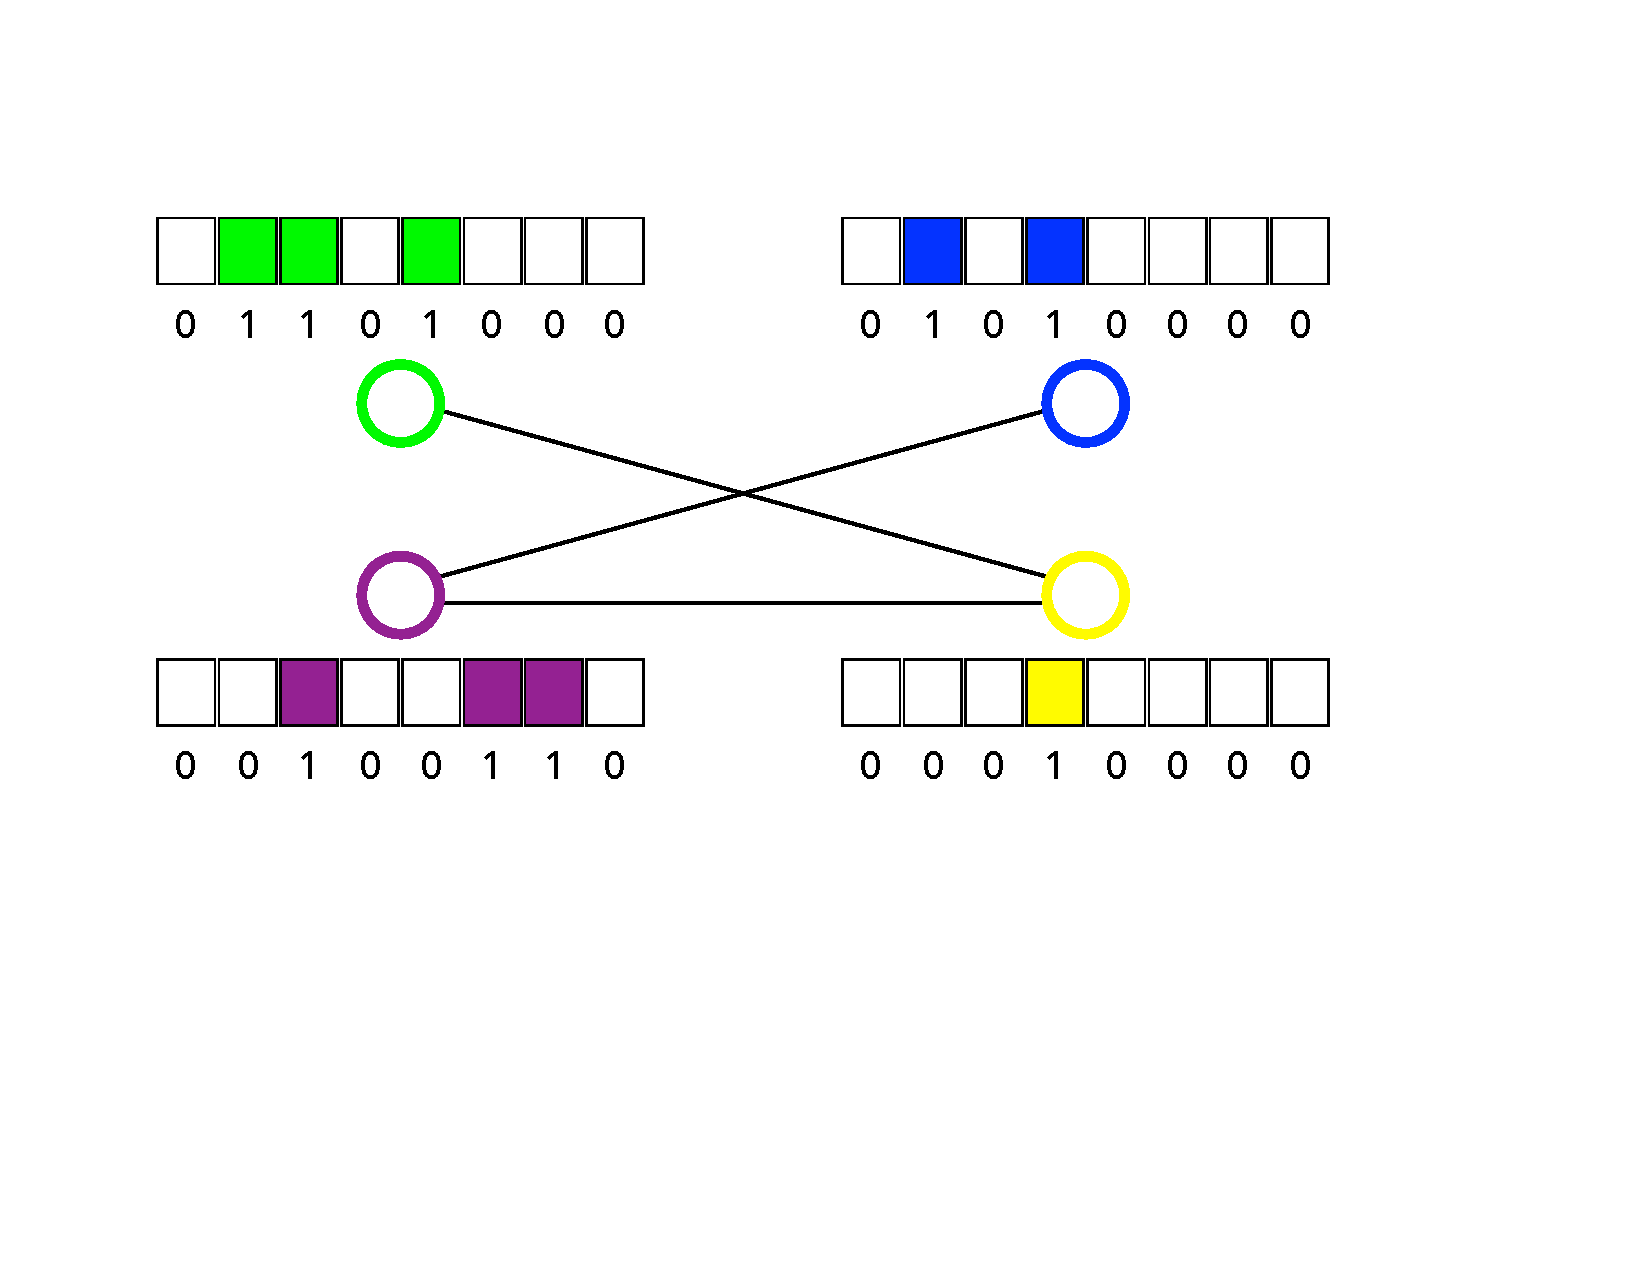
\includegraphics[width=.5\textwidth]{Chapters/mesh/figures/graph-diagram.pdf}
%  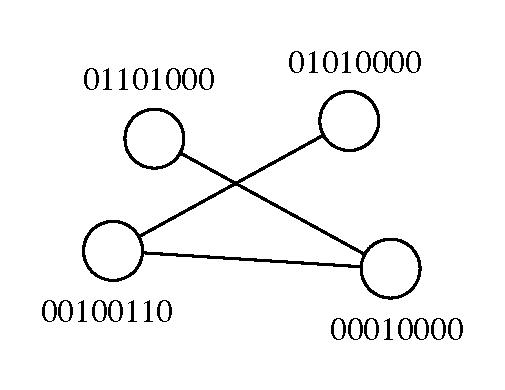
\includegraphics[width=.33\textwidth]{figures/meshing_graph.pdf}
%  \vspace{-2em}
%\centering
\caption{\textbf{An example meshing graph.}  Nodes correspond to the spans represented by the strings \texttt{01101000}, \texttt{01010000}, \texttt{00100110}, and \texttt{00010000}.  Edges connect meshable strings (corresponding to non-overlapping spans).}\label{fig:exmesh}
\end{figure}


\subsection{Formal Problem Definitions}
\label{subsec:probdef}
Since \Mesh{} segregates objects based on size, we can limit our
analysis to compaction within a single size class without loss of
generality. For our analysis, we represent spans as binary strings of
length $b$, the maximum number of objects that the span can
store. Each bit represents the allocation state of a single object. We
represent each span $\page$ with string $\str$ such that $\str\lp
i\rparen = 1$ if $\page$ has an object at offset $i$, and 0 otherwise.

\begin{definition}
We say  two  strings $\str_{1}, \str_{2}$ \em{mesh} iff $\sum_i \str_{1}\lp i\rparen \cdot \str_{2} \lp i \rparen = 0$. More generally, a set of binary strings are said to mesh if every pair of strings in this set mesh.
%We say that k binary strings $\str_{1}, ... \str_{k}$ mesh iff $\sum_{j \in [1,k]} \str_{j}(i) \leq 1$ $\forall i \in [0,b-1]$.\\
%Equivalently, k binary strings mesh if each each of said strings are pairwise meshable with all of the other strings.
\end{definition}

When we mesh $k$ spans together, the objects scattered across those
$k$ spans are moved to a single span while retaining their offset from
the start of the span. The remaining $k-1$ spans are no longer needed
and are released to the operating system. We say that we ``release''
$k-1$ \emph{strings} when we mesh $k$ strings together.  Since our
goal is to empty as many physical spans as possible, we can
characterize our theoretical problem as follows:

\begin{problem}
Given a multi-set of $n$ binary strings of length $b$, find a meshing
that releases the maximum number of strings.
\end{problem}

% Note that the total number of strings released is equal to $n - \rho -
% \phi$, where $\rho$ is the number of total meshes performed, and $\phi$
% is the number of strings that remain unmeshed.

\paragraph{A Formulation via Graphs:}
\label{subsec:graph}

We observe that an instance of the meshing problem, a string multi-set
$S$, can naturally be expressed via a graph $G(S)$ where there is a
node for every string in $S$ and an edge between two nodes iff the
relevant strings can be meshed. Figure~\ref{fig:exmesh} illustrates
this representation via an example.

%Given , we construct a meshing graph $G_S$ as follows:\\
%We add a node $\node$ to $G_S$ for each $\str \in S$.  We say node $\node$ represents $\str$.  For each %node pair $\node_1, \node_2$, we add edge $(\node_1, \node_2)$ iff $\node_1$ and $\node_2$ mesh.

%This meshing problem is reducible to min clique cover (MCC), an NP-Complete problem.  We implicitly show %this reduction through a straightforward graph interpretation of the meshing problem.

If a set of strings are meshable, then there is an edge between every
pair of the corresponding nodes: the set of corresponding nodes is a
\emph{clique}. We can therefore decompose the graph into $k$ disjoint
cliques iff we can free $n-k$ strings in the meshing
problem. Unfortunately, the problem of decomposing a graph into the
minimum number of disjoint cliques (\textsc{MinCliqueCover}) is in
general NP-hard. Worse, it cannot even be approximated up to a factor
$m^{1-\epsilon}$ unless $P=NP$~\cite{zuckerman07}.

While the meshing problem is reducible to {\textsc{MinCliqueCover}},
we have not shown that the meshing problem is NP-Hard.  The meshing
problem is indeed NP-hard for strings of arbitrary length, but in
practice string length is proportional to span size, which is
constant.

\begin{theorem}\label{thm:polytime}
The meshing problem for $S$, a multi-set of strings of constant length, is in $P$. %can be solved in polynomial time.
%is in P
%; equivalently, the min clique cover problem on meshing graphs generated from sets of strings of constant %length is in P.
\end{theorem}

\begin{proof}
We assume without loss of generality that $S$ does not contain the
all-zero string $\str_0$; if it does, since $\str_0$ can be meshed
with any other string and so can always be released, we can solve the
meshing problem for $S \setminus \str_0$ and then mesh each instance
of $\str_0$ arbitrarily.

Rather than reason about {\textsc{MinCliqueCover}} on a
 meshing graph $G$, we consider the equivalent
problem of coloring the complement graph $\bar{G}$ in which there is
an edge between every pair of two nodes whose strings do not mesh. The nodes of $\bar{G}$ can be partitioned into at most $2^b-1$
subsets $N_1 \ldots N_{2^b-1}$ such that all nodes in each
$N_i$ represent the same string $\str_i$.  The induced subgraph of
$N_i$ in $\bar{G}$ is a clique since all its nodes have a 1 in the same position and so cannot be pairwise meshed.  Further, all nodes in $N_i$ have the same set of neighbors.

Since $N_i$ is a clique, at most one node in $N_i$ may be colored with
any color.  Fix some coloring on $\bar{G}$.  Swapping the colors of
two nodes in $N_i$ does not change the validity of the coloring since
these nodes have the same neighbor set.  We can therefore
unambiguously represent a valid coloring of $\bar{G}$ merely by
indicating in which cliques each color appears.

With $2^b$ cliques and a maximum of $n$ colors, there are at most $\lp
n+1 \rparen ^{c}$ such colorings on the graph where $c=2^{2^b}$. This follows because each color used can be associated with a subset of $\{1, \ldots, 2^b\}$ corresponding to which of the cliques have node with this color; we call this subset a \emph{signature} and note there are $c$ possible signatures. A coloring can be therefore be associated with a multi-set of possible signatures where each signature has multiplicity between 0 and $n$; there are $(n+1)^c$ such multi-sets. This is polynomial in $n$ since $b$ is constant and hence $c$ is also constant. So we can simply check each coloring for validity (a coloring is valid iff no color appears in two cliques whose string representations mesh). The algorithm returns a valid coloring with the lowest number of colors from all valid colorings discovered.
\end{proof}

%Unfortunately, the exponent of $n$ runtime grows doubly exponentially in  $b$ and $b$ can be as large as 256.
%Such a runtime,
Note that the runtime of the above algorithm is at least exponential in the string length. While technically polynomial for constant string length, the running time of the above algorithm would obviously be prohibitive in practice and so we never employ it in \Mesh{}. Fortunately, as we show next, we can exploit the randomness in the strings to design a much faster algorithm.

\subsection{Simplifying the Problem: From \textsc{MinCliqueCover} to \textsc{Matching}}
\label{subsec:matching}
We leverage \Mesh{}'s random allocation to simplify meshing; this random
allocation implies a distribution over the graphs that exhibits useful
structural properties. We first make the following important observation:

\begin{observation}
Conditioned on the occupancies of the strings, edges in the meshing graph  are not three-wise independent.
\end{observation}

To see that edges are not three-wise independent consider three random
strings $s_1, s_2, s_3$ of length 4, each with exactly 2 ones. It is
impossible for these strings to all mesh mutually since if we know that $s_1$ and $s_2$ mesh,
and that $s_2$ and $s_3$ mesh, we know for certain that $s_1$ and
$s_3$ cannot mesh. More generally, conditioning on $s_1$ and $s_2$
meshing and $s_1$ and $s_3$ meshing decreases the probability that
$s_1$ and $s_3$ mesh.
%Note that even when we assume bits are 1 or 0
%independently, edges are still not independent.
%The existence of edge
%($s_4,s_5$) is weak evidence of $s_5$'s low occupancy, increasing the
%probability that edge ($s_5,s_6$) exists.
Below, we quantify this
effect to argue that we can mesh near-optimally by solving the much
easier \textsc{Matching} problem on the meshing graph (i.e.,
restricting our attention to finding cliques of size 2) instead of
\textsc{MinCliqueCover}. Another consequence of the above observation is that we will not be able to appeal to  theoretical results on the standard model of random graphs, \emph{Erd\H{o}s-Renyi graphs}, in which  each possible edge is present with some fixed probability and the edges are fully independent. Instead we will need new algorithms and proofs that only require independence of acyclic collections of edges.

\paragraph{Triangles and Larger Cliques are Uncommon.}
Because of the dependencies across the edges present in a meshing
graph, we can argue that \emph{triangles} (and hence also larger
cliques) are relatively infrequent in the graph and certainly less
frequent than one would expect were all edges independent.  For
example, consider three strings $s_1, s_2, s_3\in \{0,1\}^b$ with
occupancies $r_1, r_2,$ and $r_3$, respectively. The probability they
mesh is
\[
{\binom{b-r_1}{r_2}} \big / {\binom{b}{r_2}} \times {\binom{b-r_{1}-r_2 }{r_3}} \big / {\binom{b}{r_3}} \ . \]

This value is significantly less than would have been the case if the
events corresponding to pairs of strings being meshable were
independent.
%In most practical cases, we will not be interested in meshing strings with low occupancy --- it is often better just to wait until %the last objects on these spans are freed.  For higher occupancies, the expected number of triangles is quite low.
For instance, if $b = 32, r_1=r_2=r_3 = 10$, this probability is so
low that even if there were $1000$ strings, the expected number of
triangles would be less than 2. In contrast, had all meshes been
independent, with the same parameters, there would have been $167$ triangles.

% \paragraph{We Can Restrict Our Attention to Matching.}
\begin{comment}
The above analysis leads us to conclude that, since there are
relatively few triangles in meshing graphs, we can achieve almost the
full benefits of solving \textsc{MinCliqueCover} by only solving
\textsc{Matching}.
\end{comment}

The above analysis suggests that we can focus on finding only cliques
of size 2, thereby solving \textsc{Matching} instead of
\textsc{MinCliqueCover}. The evaluation in
Section~\ref{sec:evaluation} vindicates this approach, and we show a
strong accuracy guarantee for \textsc{Matching} below.
% We also verify this empirically in the Appendix.

\subsection{Theoretical Guarantees}
\label{subsec:analysis}
Since we need to perform meshing at runtime, it is essential that our
algorithm for finding strings to mesh be as efficient as possible. It
would be far too costly in both time and memory overhead to actually
construct the meshing graph and run an existing matching algorithm on
it. Instead, the \sm algorithm (shown in Figure \ref{fig:meshalg})
performs meshing without the need for explicitly constructing the
meshing graph.

For further efficiency, we need to constrain the value of the
parameter $t$, which controls \Mesh{}'s space-time tradeoff. If $t$
were set as large as $n$, then \sm could, in the worst case,
exhaustively search all pairs of spans between the left and right
sets: a total of $n^2/4$ probes.  In practice, we want to choose a
significantly smaller value for $t$ so that \Mesh{} can always
complete the meshing process quickly without the need to search all
possible pairs of strings.


\begin{lemma}
Let $t=k/q$ where $k>1$ is some user defined parameter and $q$ is the global probability of two
spans meshing. \sm finds a matching
of size at least $n(1-e^{-2k})/4$ between the left and right span sets
with probability approaching 1 as $n\geq 2k/q$ grows.
\end{lemma}

\begin{proof}
%\sm in essence creates a bipartite meshing graph by splitting the span set in half.
Let $S_l=\{v_1, v_2, \ldots v_{n/2}\}$ and $S_r=\{u_1,
u_2, \ldots u_{n/2}\}$. Let $t=k/q$ where
$k>1$ is some arbitrary constant. For $u_i\in S_l$ and $i \leq j \leq
j+t$, we say $(u_i,v_j)$ is a \emph{good match} if all the following
properties hold: (1) there is an edge between $u_i$ and $v_j$, (2)
there are no edges between $u_i$ and $v_{j'}$ for $i\leq j'<j$, and
(3) there are no edges between $u_{i'}$ and $v_{j}$ for $i< i'\leq j$.

We observe that \sm finds any good match, although it may
also find additional matches. It therefore suffices to consider only
the number of good matches. The probability $(u_i,v_j)$ is a good
match is $q(1-q)^{2(j-i)}$ by appealing to the fact that the collection of edges under consideration is acyclic. Hence, $\Pr(u_i \mbox{ has a good match})$
is
\begin{align*}
r:= q \sum_{i=0}^{k/q-1} \lp 1-q\rparen ^{2i} = q \frac{1-(1-q)^{2k/q}}{1-(1-q)^2}
% \geq q \frac{1-e^{-2k}}{2q-q^2}
 > \frac{1-e^{-2k}}{2} \ .
\end{align*}

To analyze the number of good matches, define $X_i = 1$ iff $u_i$ has
a good match. Then, $\sum_i X_i$ is the number of good matches. By
linearity of expectation, the expected number of good matches is
$rn/2$. We decompose $\sum_i X_i$ into \[Z_0+Z_1+\ldots + Z_{t-1} ~~\mbox{
  where }~~ Z_{j} = \sum_{i\equiv j \bmod t} X_i \ .\] Since each
$Z_j$ is a sum of $n/(2t)$ independent variables, by the Chernoff
bound, $P\lp Z_j < \lp 1-\epsilon \rparen E[Z_j]\rparen \leq \exp\lp -
\epsilon^2 r n/(4t)\rparen$.  By the union bound,
$$P\lp X < \lp 1-\epsilon \rparen rn/2\rparen \leq t \exp\lp - \epsilon^2 r
n/(4t)\rparen$$ and this becomes arbitrarily small as $n$ grows.
\end{proof}

In the worst case, the algorithm checks $nk/2q$ pairs. For our
implementation of \Mesh, we use a static value of $t = 64$; this value
enables the guarantees of Lemma 5.1 in cases where significant meshing
is possible.  As Section~\ref{sec:evaluation} shows, this value for
$t$ results in effective memory compaction with modest performance
overhead.



\begin{comment}

\subsection{New Lower Bound for Maximum Matching Size}
\label{subsec:lowerbound}

In this section, we develop a bound for the size of the maximum matching in a graph that can easily be estimated in the context of meshing graphs.  As meshing may be costly to perform, this lower bound is useful as it can be used to predict the magnitude of compaction achievable before committing to the process.  In the case where little compaction is possible, it is often better not to try to mesh and instead conserve resources for other tasks. The quantity we introduce will always lower bound the size of  the maximum matching and will typically be relatively close to the size of the maximum matching.  For example, if we want to release 30\% of our active spans through meshing, but the bound suggests a release of less than 5\% is possible, we can infer that the maximum matching on the graph is small and meshing is currently not worth attempting.

Our approach is based on extending a result by McGregor and Vorotnikova \cite{McGregorV16}. Let $\ndegree(u)$ be the degree of node $u$ in a graph. They considered the quantity
$\sum_{e\in E} 1/\max(\ndegree(u),\ndegree(v))$
and showed that it is at most a factor $3/2$ larger than the maximum matching in the graph and at most a factor $4$ smaller in the case of planar graphs. These bounds were tight.  For example, on a complete graph on three nodes, the quantity is $3/2$ while $M$ is 1. Meshing graphs are very unlikely to be planar but are likely be almost regular, i.e., most degrees are roughly similar.
We need to extend the above bound such that we can guarantee that it never exceeds the size of the maximum matching while also being a good estimate for the graphs that are likely to arise as meshing graphs.

%\begin{theorem}
%Define $W(G)$ to be a fractional matching on graph $G = (V,E)$ such that $$W = \sum_{(u,v) \in E} \min\lp %\frac{1}{\ndegree\lp u\rparen },\frac{1}{\ndegree\lp v\rparen }\rparen $$
%Then $W\leq \frac{3}{2} M$ where $M$ is the cardinality of the maximum matching on $G$.
%If $G$ is bipartite, then $W \leq M$.
%\end{theorem}

%For general graphs, $W$ is not always a lower bound on the maximum matching (hence the need for the $\frac{3}{2}$ factor).  For example, on a complete graph on three nodes, $W$ is $\frac{3}{2}$ while $M$ is 1.

%\begin{figure}[h]
%\includegraphics[scale = .7]{figures/triangle_matching.png}
%\centering
%\caption{W is not a lower bound for the maximum matching on a triangle.}
%\end{figure}
One simple approach is to scale the above quantity by a factor of $2/3$,
but this can result in a poor approximation for the size of the
maximum matching for some graphs of interest. Instead, we take a more
nuanced approach. Specifically, we prove the following theorem (proof omitted
due to space constraints):
%in the
%Appendix:

%While it is tight for this example, for larger non-bipartite graphs it seems like scaling $W$ down by %$\frac{2}{3}$ is overkill.  For instance, for a complete graph on an odd number of nodes k, $W = %{{k}\choose{2}} \frac{1}{k-1} = \frac{k}{2}$, while $M = \frac{k-1}{2}$.
%The following theorem provides a tight lower bound for this example.


\begin{theorem}
\[
\W=\sum_{e\in E} \frac{1}{\max(\ndegree(u), \ndegree(v))+I[\min(\ndegree(u),\ndegree(v))>1]}\leq M \ .
\]
%where $f(1,\cdot)=f(\cdot,1)=f(2,3)=f(3,2)=0$ and $f(\cdot,\cdot)=1$ otherwise. Then, $\sum_{e\in E} w_e \leq M$.
% . Then, $\sum_{e\in E} w_e \leq M$.
\end{theorem}

\paragraph{A remark on estimating $\W$.}  If we wish to use this lower bound to decide whether to begin meshing by predicting the size of the maximum matching, we cannot compute it exactly because we do not know the degrees of the nodes in the graph.  However, we do know the degree distribution of the graph and so it is possible to calculate the expected value of $\W$.

\end{comment}



%\subsection{Summary}
%\label{subsec:theorysummary}

\subsection{Summary of Analytical Results}
We show the problem of meshing is reducible to a graph problem,
\textsc{MinCliqueCover}.  While solving this problem is infeasible, we
show that probabilistically, we can do nearly as well by finding the
maximum \textsc{Matching}, a much easier graph problem. We analyze our
meshing algorithm as an approximation to the maximum matching on a
random meshing graph, and argue that it succeeds with high
probability.
%Finally, we prove a new lower bound on the maximum matching for graphs
%based on degree distribution.
As a corollary of these results, \Mesh breaks the Robson
bounds with high probability.

%for a broad class of applications.
%As long as programs do not alter
%programs that do not alter their allocation behavior in response to
%addresses the allocator returns.


\begin{comment}
  An adversary attempting to create an
unmeshable memory state requires the capability to position objects at
the same locations in multiple spans.  But an address-oblivious
adversary can only do this with low probability - since allocation
offsets within a span are random, the best it can do is free some
objects from each span and hope that some of the remaining objects
reside at the same offset.  Since objects are distributed uniformly at
random from within spans, our analytical results hold and therefore
there is either a large maximum matching on the resulting meshing
graph (indicating significant compaction is possible) or spans are so
full that fragmentation is not significant.
\end{comment}


\section{Summary of Evaluation}
\label{sec:evaluation}
For a number of memory-intensive applications, including aggressively
space-optimized applications like Firefox, \Mesh can substantially
reduce memory consumption (by 16\% to 39\%) while imposing a modest
impact on runtime performance (e.g., around 1\% for Firefox and
SPECint 2006). We find that \Mesh{}'s randomization can enable
substantial space reduction in the face of a regular allocation
pattern.


%\section{Discussion}
%\label{sec:discussion}
%...


\section{Related Work}
\label{sec:related-work}

\paragraph*{Hound:}
\label{sec:hound}
Hound is a memory leak detector for C/C++ applications that introduced
meshing (a.k.a. ``virtual compaction''), a mechanism that \Mesh{}
leverages~\cite{1542521}. Hound combines an age-segregated heap with
data sampling to precisely identify leaks. Because Hound cannot
reclaim memory until every object on a page is freed, it relies on a
heuristic version of meshing to prevent catastrophic memory
consumption. Hound is unsuitable as a replacement general-purpose
allocator; it lacks both \Mesh's theoretical guarantees and space and
runtime efficiency (Hound's repository is missing files and it does
not build, precluding a direct empirical comparison here). The Hound
paper reports a geometric mean slowdown of $\approx 30\%$ for
SPECint2006 (compared to \Mesh{}'s 0.7\%), slowing one benchmark
(\texttt{xalancbmk}) by almost $10\times$. Hound also generally
\emph{increases} memory consumption, while \Mesh often substantially
decreases it.

%Finally, Hound was designed for
%32-bit Linux applications, making more direct comparisons to Mesh
%(which is focused on 64-bit applications) hard.


\paragraph*{Compaction for C/C++:}
Previous work has described a variety of manual and compiler-based
approaches to support compaction for C++. Detlefs shows that if
developers use annotations in the form of smart pointers, C++ code can
also be managed with a relocating garbage
collector~\cite{detlefs:1992:gc}.  Edelson introduced GC support
through a combination of automatically generated smart pointer classes
and compiler transformations that support relocating
GC~\cite{edelson:1992:precompilingcgc}. Google's Chrome uses an
application-specific compacting GC for C++ objects called Oilpan that
depends on the presence of a single event
loop~\cite{google:oilpan}. Developers must use a variety of smart
pointer classes instead of raw pointers to enable GC and
relocation. This effort took years. Unlike these approaches, \Mesh is
fully general, works for unmodified C and C++ binaries, and does not
require programmer or compiler support; its compaction approach is
orthogonal to GC.

CouchDB and Redis implement \emph{ad hoc} best-effort compaction,
which they call ``defragmentation''.  These work by iterating through
program data structures like hash tables, copying each object's
contents into freshly-allocated blocks (in the hope they will be
contiguous), updating pointers, and then freeing the old
objects~\cite{jemalloc:exposehints,redis:announcement}. This
application-specific approach is not only inefficient (because it may
copy objects that are already densely packed) and brittle (because it
relies on internal allocator behavior that may change in new
releases), but it may also be ineffective, since the allocator cannot
ensure that these objects are actually contiguous in memory. Unlike
these approaches, \Mesh performs compaction efficiently and its
effectiveness is guaranteed.

\paragraph*{Compacting garbage collection in managed languages:}
%% Recently Baker et al. showed that with compiler support you could
%% achieve accurate GC for C and C++~\cite{baker:2009:accurategc}.
Compacting garbage collection has long been a feature of languages
like LISP and
Java~\cite{hansen:1969:compaction,fenichel:1969:compaction}. Contemporary
runtimes like the Hotspot JVM~\cite{microystems2006memory}, the .NET
VM~\cite{microsoft:dotnet-gc}, and the SpiderMonkey JavaScript
VM~\cite{mozilla:spidermonkey-compaction} all implement compaction as
part of their garbage collection algorithms. \Mesh{} brings the
benefits of compaction to C/C++; in principle, it could also be used
to automatically enable compaction for language implementations that
rely on non-compacting collectors.

\paragraph*{Bounds on Partial Compaction:}
Cohen and Petrank prove upper and lower bounds on defragmentation via
partial compaction~\cite{Cohen:2017:LPC:3050768.2994597,
  Cohen:2013:LPC:2491956.2491973}. In their setting, corresponding to
managed environments, \emph{every} object \emph{may} be relocated to
any free memory location; they ask what space savings can be achieved
if the memory manager is only allowed to relocate a bounded number of
objects. By contrast, \Mesh{} is designed for unmanaged languages
where objects \emph{cannot} be arbitrarily relocated.

%\paragraph{Hardware support:}
%Seshadri \emph{et al.} present a hardware proposal that would allow
%for ``page overlays'' at a cache-line
%granularity~\cite{Seshadri:2015:POE:2749469.2750379}. \Mesh could use
%such a facility instead of page remapping to mesh pages containing
%objects of a cache line size (e.g., 64 bytes) or larger.

\paragraph*{PCM fault mitigation:}
Ipek \emph{et al.} use a technique similar to meshing to address the
degradation of phase-change memory (PCM) over the lifetime of a
device~\cite{ipek:2010:dynamic-replication}.  The authors introduce
dynamically replicated memory (DRM), which uses pairs of PCM pages
with non-overlapping bit failures to act as a single page of
(non-faulty) storage.  When the memory controller reports a page with
new bit failures, the OS attempts to pair it with a complementary
page. A random graph analysis is used to justify this greedy
algorithm.

DRM operates in a qualitatively different domain than \Mesh.  In DRM,
the OS occasionally attempts to pair newly faulty pages
against a list of pages with static bit failures.  This process is
incremental and local.  In \Mesh, the occupancy of spans in the heap
is more dynamic and much less local. \Mesh solves a full,
non-incremental version of the meshing problem each cycle.
Additionally, in DRM, the random graph describes an error model rather
than a design decision; additionally, the paper's analysis is flawed.
The paper erroneously claims that the resulting graph is a simple
random graph; in fact, its edges are not independent (as we show in
\S\ref{subsec:matching}).  This invalidates the claimed performance
guarantees, which depend on properties of simple random graphs. In
contrast, we prove the efficacy of our original \sm algorithm for
\Mesh using a careful random graph analysis.

\begin{comment}
  To avoid catastrophic memory consumption,
Hound employs virtual compaction, a non-randomized, best-effort form
of meshing. Their approach depends on heuristics and does not employ
randomization or come with any guarantees of fragmentation
recovery.
  Hound is not intended to be
space-efficient (and it is not) but rather to find leaks. Hound
identifies leaks by segregating objects by allocation site, protects
``cold'' pages, and delays reuse of pages until every object on that
page has been freed.
\end{comment}

%% Virtual memory operations have additionally been use for compaction in
%% a Java garbage collector~\cite{wegiel:2008:mapping-collector} in a
%% novel collector, as well as in a C allocator that traded address space
%% usage for reliability and security~\cite{1346296}.

%Microsoft's C++/CLI? C++ with GC'ed, moveable objects.


% http://www.filpizlo.com/papers/baker-ccpe09-accurate.pdf


%Theory?

%% Objects with similar lifetimes tend to appear
%% together~\cite{wilson:1995:survey}.


\section{Conclusion}
\label{sec:conclusion}

This chapter introduces \Mesh{}, a memory allocator that efficiently
performs \textit{compaction without relocation} to save memory for
unmanaged languages.  We show analytically that \Mesh{} provably
avoids catastrophic memory fragmentation with high probability, and
empirically show that \Mesh{} can substantially reduce memory
fragmentation for memory-intensive applications written in C/C++ with
low runtime overhead. In future work, we plan to
explore integrating \Mesh{} into language runtimes that do not
currently support compaction, such as Go and Rust.

We have released \Mesh as an open source
project; it can be used with arbitrary C and C++ Linux and Mac OS X
binaries and can be downloaded at
\url{http://libmesh.org}.


\iffalse

%% contents suppressed with 'anonymous'
\begin{acks}
  %% Commands \grantsponsor{<sponsorID>}{<name>}{<url>} and
  %% \grantnum[<url>]{<sponsorID>}{<number>} should be used to
  %% acknowledge financial support and will be used by metadata
  %% extraction tools.
  This material is based upon work supported by the
  \grantsponsor{GS100000001}{National Science
    Foundation}{http://dx.doi.org/10.13039/100000001} under Grant
  No.~\grantnum{GS100000001}{1637536}.  Any opinions, findings, and
  conclusions or recommendations expressed in this material are those
  of the author and do not necessarily reflect the views of the
  National Science Foundation.
\end{acks}

\fi

%\bibliography{Chapters/mesh/emery,Chapters/mesh/mesh}

%% \clearpage
%% \pagebreak
\section{Appendix}
\label{sec:appendix}
\newtheorem*{remark}{Remark}

\newcommand{\rp}{\right)}


% TODO: reorganize!

\subsection{Proof of Theorem \ref{thm:polytime}}

\begin{comment}
\begin{proof}
We assume without loss of generality that $S$ does not contain the all-zero string $\str_0$; if it does, since $\str_0$ can be meshed with any other string and so can always be released, we can solve the meshing problem for $S \setminus \str_0$ and then mesh each instance of $\str_0$ arbitrarily.

Rather than reason directly about the Min Clique Cover problem on some bounded-length meshing graph $G$, let us consider the equivalent problem of coloring $\bar{G}$, the complement of $G$.  $\bar{G}$ has an edge between  every pair of two nodes whose strings do not mesh.

$\bar{G}$'s node set $N$ can be partitioned into at most $2^b-1$ subsets $N_1, N_2, ... N_{2^b-1}$ such that $\forall i$, all nodes in $N_i$ represent the same string $\str_i$.  The induced subgraph of $N_i$ is a clique since all its nodes have a 1 in the same position and so cannot be pairwise meshed.  Further, all nodes in $N_i$ has the same neighbors since they all represent the same string.

Since $N_i$ is a clique, at most one node in $N_i$ may be colored with any color.  Fix some coloring on $\bar{G}$.  Swapping the colors of two nodes in $N_i$ does not change the validity of the coloring since these nodes have the same neighbor set.  We can therefore unambiguously represent a valid coloring of $\bar{G}$ merely by indicating in which cliques each color appears.

With $2^b$ cliques and a maximum of $n$ colors, there are at most $\lp n+1 \rp ^{2^{2^b}}$ such colorings on the graph.  This is polynomial in $n$ since $b$ is fixed, so we can simply check each coloring for validity (a coloring is valid iff no color appears in two cliques whose string representations mesh).  Finally, the algorithm returns a valid coloring with the lowest number of colors out of all valid colorings discovered.
\end{proof}
\end{comment}


We assume without loss of generality that $S$ does not contain the all-zero string $\str_0$; if it does, since $\str_0$ can be meshed with any other string and so can always be released, we can solve the meshing problem for $S \setminus \str_0$ and then mesh each instance of $\str_0$ arbitrarily.

Let $\bar G = (V, \bar E)$ be the complement of $G$.  Solving \textsc{MinCliqueCover} on $G(S)$ is equivalent to solving \textsc{Coloring} on $\bar G$.

\begin{lemma}
There are a polynomial number of colorings on $\bar G$.
\end{lemma}
\begin{proof}
Partition $V$ into $V_1, V_2, ... V_k$ such that $V_i = \{u \vert str(u) = s_i\}$.  Note that the induced subgraph of $\bar G$ on each $V_i$ is a clique, and further that $k \leq 2^b-1$.

Since $V_i$ is a clique, at most one node in $V_i$ may be colored with any color.  Fix some coloring on $\bar{G}$.  Swapping the colors of two nodes in $V_i$ does not change the validity of the coloring since these nodes have the same neighbor set.  We can therefore unambiguously represent a valid coloring of $\bar{G}$ merely by indicating in which cliques each color appears.

With $2^b$ cliques and a maximum of $|V| = n$ colors, there are at most $\lp n+1 \rp ^{2^{2^b}}$ such colorings on the graph.
\end{proof}

As a result of the lemma, we can check all colorings in polynomial time and return the minimum valid coloring.

\begin{remark}
This proof relies on the assumption that $b$, string length, is fixed.  This constraint limits meshing graphs to a strict subset of all possible graphs.  If $b = \bigo(n^2)$, any graph can be expressed as a meshing graph and so \textsc{MinCliqueCover} is NP-Hard in this case.
\end{remark}

\subsection{Experimental Confirmation of Maximum Matching/Min Clique Cover Convergence}

In Section~\ref{subsec:matching}, we argue that we can approximate the solution to \textsc{MinCliqueCover} on meshing graphs with high probability by instead solving \textsc{MaximumMatching}.

We experimentally verify this result by generating many random constant occupancy graphs and, for each graph, comparing the size of the maximum matching to the size of a greedy (non-optimal) solution for \textsc{MinCliqueCover}.  The results are summarized in Figure~\ref{plot:const}.

\begin{figure}[h]
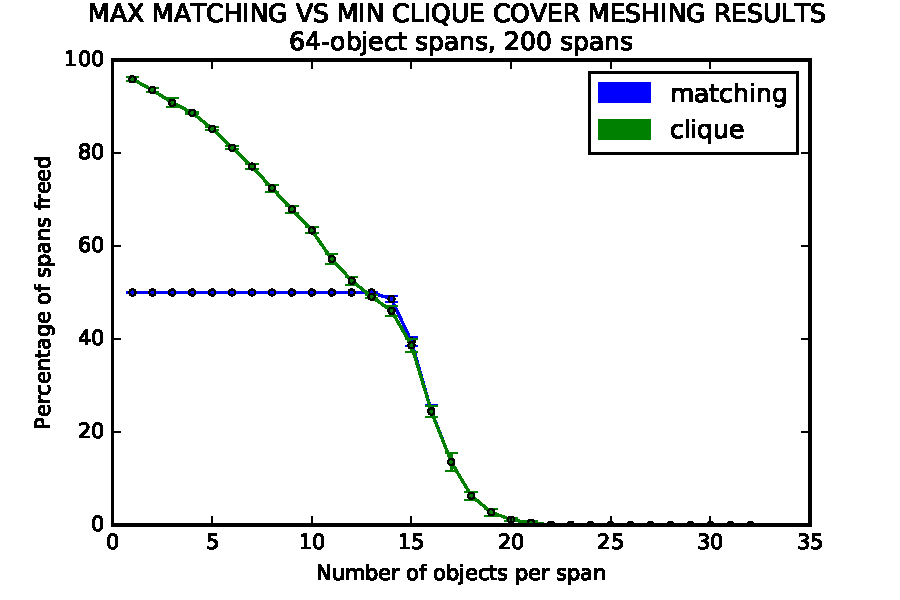
\includegraphics[scale = .5]{figures/const_match_comp.pdf}
\centering
\caption{\textbf{Min Clique Cover and Max Matching solutions converge.} The average size of Min Clique Cover and Max Matching for randomly generated constant occupancy meshing graphs, plotted against span occupancy.  Note that for sufficiently high-occupancy spans, Min Clique Cover and Max Matching are nearly equal.}
\label{plot:const}
\end{figure}



When we instead assume bits are 1 independently with probability p, we expect the graph to have many more triangles.  For $p = r/b = 10/32, n = 1000$, the expected number of triangles is roughly 36,000.  However, we can see experimentally that these graphs behave quite similarly in Figure~\ref{plot:indep}.


\begin{figure}[h]
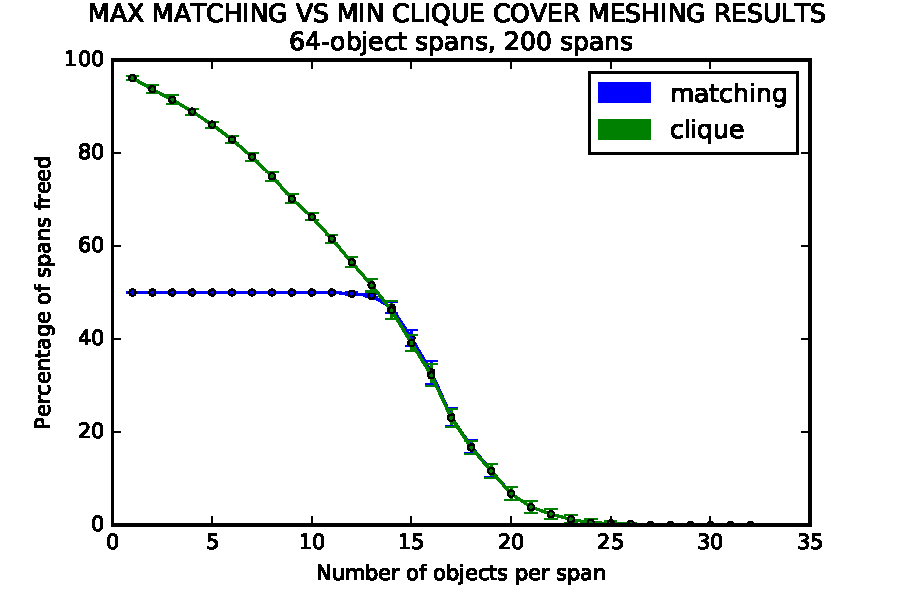
\includegraphics[scale = .5]{figures/ind_match_comp.pdf}
\centering
\caption{\textbf{Converge still holds for independent bits assumption.} The average size of Min Clique Cover and Max Matching for randomly generated constant occupancy meshing graphs, plotted against span occupancy.  Note that for sufficiently high-occupancy spans, Min Clique Cover and Max Matching are nearly equal.}
\label{plot:indep}
\end{figure}

While constant occupancy graphs are fairly regular, independent bit graphs may not be.  Since strings have different occupancies, nodes which correspond to strings with relatively low occupancy will tend to have significantly higher degree than other nodes in the graph.  Meanwhile, other nodes may have strings with high occupancy, and therefore only have a few edges (probably with low-occupancy nodes).  So while there are many triangles, when the graph is sparse enough, even meshing cliques of size 3 and 4 will likely "abandon" adjacent high-occupancy nodes, one of which could have been matched with the high degree node to yield the same number of releases.

So in this case we still expect finding the maximum matching to be good enough.

\iffalse
\subsection{Proof of Theorem 4.4}
\begin{proof}
Since spans all have identical occupancies, we expect the meshing graph to be nearly regular - the degree of each node is binomially distributed with mean $\lp n-1\rp q$.  When there are many objects per span, the degree distribution will be tightly concentrated around this mean.  For example, when $b = 128, n = 1000, q = .05$, the mean degree is 50 and less than 5\% of nodes have a degree greater than 60.

When we split the span set into half, and only consider pairs between the halves, we essentially remove half of the edges from the meshing graph.  To see this, observe that there are ${{n}\choose{2}} \approx n^2/2$ span pairs, and we fail to consider $2*{{n/2}\choose{2}} \approx n^2/4$ of them.  Note also that we fail to consider exactly $n/2 -1$ pairs for each span.  We therefore expect both the total number of edges in the meshing graph and the degree of each node to decrease by half.

How does the maximum matching of a graph change when you evenly sparsify the graph by half?  If the average degree is high enough, we expect this to not make much difference at all - each node in expectation still has many edges from which a matching can be built.

We can formalize this argument by first assuming that every node in the graph has degree at least $d$ and at most $\lp 1 + \epsilon \rp d$.  As we prove in Section~\ref{subsec:lowerbound}, the maximum matching of a graph $G = \lp V, E\rp$ is lower bounded by

$$W\lp G \rp = \sum_{\lp u,v \rp \in V} \min \lp \frac{1}{\degree \lp u \rp +1}, \frac{1}{\degree \lp v \rp +1} \rp$$

With our degree assumption we can further argue

\begin{align*}
W\lp G \rp \geq \sum_{\lp u,v \rp \in V} \frac{1}{\lp 1+\epsilon \rp d+1}
 \geq \frac{nd/2}{\lp 1+\epsilon \rp d+1}
\geq \frac{n}{2\lp 1+\epsilon \rp}
\end{align*}
and $W\leq n/2$.
%\lp G \rp &\leq \sum_{\lp u,v \rp \in V} \frac{1}{d+1} \leq \frac{n}{2}$
%\begin{align*}
%W\lp G \rp &\leq \sum_{\lp u,v \rp \in V} \frac{1}{d+1} \leq \frac{n}{2}
%\end{align*}

Note how these upper and lower bounds are independent of $d$ and $m$.  Thus, we decrease the maximum matching by at most a $1/\lp 1+\epsilon \rp$ factor by splitting the span set.
\end{proof}
\fi

\subsection{Proof of Theorem 4.5}
\begin{proof}
We begin by showing that the simpler quantity $W$ is a lower bound of the maximum matching $M$.
\[
W = \sum_{e\in E} \frac{1}{\max(\degree\lp u\rp, \degree\lp v\rp )+1}\ .
\]
%For each edge $e = (u,v) \in G$, define $\W$$(e)=min\lp \frac{1}{\degree\lp u\rp +1},\frac{1}{\degree\lp %v\rp +1}\rp$.  L
Let $U$ be an arbitrary set of $t$ nodes in $G$ where $t$ is odd.   Define $$W(U) = \sum_{u,v \in U} \frac{1}{\max(\degree\lp u\rp, \degree\lp v\rp )+1} \ . $$ As a corollary of Edmonds Matching Polytope Theorem, it can be shown that $W \leq M$ if  $W(U) \leq (|U|-1)/2$. We can argue this as follows:

\begin{align*}
W(U) &= \sum_{(u,v) \in U} \min \left(\frac{1}{\degree(u)+1},\frac{1}{\degree(v)+1}\right )\\
& \leq \sum_{(u,v) \in U}\frac{1}{2}\lp \frac{1}{\degree\lp u \rp +1}+\frac{1}{\degree\lp v\rp +1}\rp\\
&\leq \sum_{(u,v) \in U}\frac{1}{2}\lp \frac{1}{\degree_U\lp u\rp +1}+\frac{1}{\degree_U\lp v\rp +1}\rp\\
&= \frac{1}{2} \sum_{u \in U} \frac{\degree_U\lp u\rp }{\degree_U\lp u\rp +1} \leq  \frac{1}{2} \lp \frac{t-1}{t}\rp  t = \frac{t-1}{2}
\end{align*}
where $\degree_U(u)$ in the number of neighbors of $u$ in the set $U$.
The second line follows from the fact that the minimum of two quantities is bounded above by their average.  The third line follows from the fact that the degree of any node in a subgraph is bounded above by its degree in the original graph.  The fourth line follows from summing over nodes instead of edges, and then reasoning that in the worst case U is a clique and so $\degree_U(u) = t-1$ for all u $u$.

\iffalse
Recall that we prove in Section~\ref{subsec:lowerbound} that when
\[
w_e=\min\lp \frac{1}{\degree\lp u\rp+1 },\frac{1}{\degree\lp v\rp+1 }\rp
~~\mbox{ and }~~\W=\sum_{e\in E} w_e \ .\]
then $\W$ is a lower bound on the cardinality of the maximum matching M(G).
\fi


In some cases $W$ is too conservative; it assigns little weight to edges which it could safely have assigned much more.  For example, if $e$ is isolated (meaning its endpoints have degree 1), $W(e) = 1/2$.  However, it is always safe to assign weight 1 to $e$, since $M(G-e) = M(G)-1.$  If we modified our rule for $W$ so that for any edge $e= (u,v)$ s.t. $\deg(u)=\deg(v) = 1$ we assigned weight $ \min(1/\deg(u),1/\deg(v))$ instead of $ \min(1/\deg(u)+1,1/\deg(v)+1)$, we would always assign weight 1 to isolated edges.

In fact, a more general rule is true.  For any edge $e= (u,v)$, if either $\deg(u) or \deg(v) = 1$ then we may assign it weight $\min(1/\deg(u),1/\deg(v))$.

\iffalse
At this point it is natural to ask whether we can remove the $+1$s from the denominator for other edges.  We cannot of course do so for $\deg(u) = \deg(v) = k >1, k \in 2\mathbb{Z}$ since for a clique on k+1 nodes this rule would result in total weight $(k+1)/2$.\\

However, we can remove the $+1$ under certain circumstances. We show that if one of the endpoints has degree one then this is the case.
\fi

%prove several rules of this form.  For each rule we specify values of $\deg(u)$ and $\deg(v)$ for which the %$+1$ can be removed from the denominator of the edge weight.
%First we restate the claim that isolated edges may safely be assigned weight 1.
%\begin{lemma}
%Define $\W(G)$ as follows:\\
%For each $(u,v) \in G$,\\
%if $\deg(u) = \deg(v) = 1$, $\W(u,v) =  \min(\frac{1}{\deg(u)},\frac{1}{\deg(v)})$.\\
%else $\W(u,v) =  \min(\frac{1}{\deg(u)+1},\frac{1}{\deg(v)+1})$.
%Then $\W(G) \leq M(G)$.
%\end{lemma}
%\begin{proof}
%Already proven above.
%\end{proof}
%Next we will amend $\W$ to include the following rule: when one endpoint has degree 1 and the other has %degree k, assign weight $\frac{1}{k}$.

Define $\W$ as follows:
\[\W=\sum_{(u,v)\in E} \W(u,v) \]
where
\[
\W(u,v)=\frac{1}{\max(\degree\lp u\rp, \degree\lp v\rp )+I[\min(\degree(u),\degree(v))> 1]}\]

We now show that $\W \leq M$. We have proven that $W(U)\leq (t-1)/2$ on any odd-size subgraph $U$, $|U| = t$.  Define subsets $U_1$ and $U_2$ of $U$ such that $U_1 \cup U_2 = U$.  $U_1$ is the set of all nodes in $U$ of degree 1 and all nodes in $U$ adjacent to a node of degree 1, and $U_2$ is the set of all other nodes in $U$.  Let $G(U_2)$ denote the subgraph of $U$ induced by $U_2$, and let $|U_1| = x$ where x is even.  Then $W(G(U_2)) = \W(G(U_2)) \leq (t-x-1)/2$.  So to complete our proof we must show that all remaining edges (call them $E'$) have total weight $\leq x/2$.

Assume WLOG that there are no isolated edges in $G$ (if there are, we can group them with $G(U_2)$ and retain the $(t-x-1)/2$ bound).

\begin{align*}
\W(E') & \leq \frac{1}{2} \sum_{u,v \in E'} \lp \frac{1}{\deg(u)}+\frac{1}{\deg(v)}\rp\\
& = \mathlarger{\sum_k} \Big(\sum_{v \in U_1, \deg(v) = k} \frac{\delta}{k} + \frac{k-\delta}{2(k+1)}\Big)
\end{align*}
where $\delta$ denotes the number of degree 1 nodes adjacent to $v$.\\
Let $f(\delta) = \delta/k + (k-\delta)/(2(k+1))$.  We are interested in finding the maximum value $f(\delta)/(\delta+1)$ can take on; if it can never take a value greater than $1/2$ then $\W(E')$ cannot be greater than $x/2$.
$$\frac{\partial\frac{f(\delta)}{\delta+1}}{\partial \delta} = \frac{2-k}{2k(\delta+1)^2}$$
which is always negative for $k \geq 2$.  So, $f(\delta)/(\delta+1)$ is maximized at $\delta = 0$, so  $f(\delta)/(\delta+1) \leq k/(2(k+1)) < 1/2.$

There is one final detail we have not considered: $x$ might be odd.  In this case, $|U_2|$ is even and we can't appeal to Theorem 3 to say that $\W(G(U_2)) \leq (t-x-1)/2$.  However, we can simply remove one node $\node'$ from $U_2$; the resulting odd-size subgraph has weight at most $(t-x-2)/2$.  Since $\W$ is a valid fractional matching, the weight assigned to all edges adjacent to $\node'$ cannot exceed 1, so we can say that $\W(G(U_2)) \leq (t-x)/2$.  Now we must show that $\W(E') \leq (x-1)/2$.

We have shown that the edge weight per node in $U_1$ cannot exceed $1/2$.  $\W(E')$ is minimized when there is exactly 1 node of degree 1, with a degree k neighbor. In this case, the only edge in $E'$ will be assigned weight $k/(2(k+1))< 1/2$.  $\W(E') \leq 1/2 + (x-2)/2 = (x-1)/2$ and the theorem is proven.
\end{proof}

\iffalse
Finally, we further amend $\W$ to include the following rule:  when one endpoint has degree 2 and the other degree 3, assign weight $\frac{1}{3}$.

\begin{lemma}
Define $\W(G)$ as follows:\\
For each $(u,v) \in G$,\\
if $\deg(u) = 1$, or if $\deg(u) = 2$ and $\deg(v) = 3$, $\W(u,v) =  \min(\frac{1}{\deg(u)},\frac{1}{\deg(v)})$.\\
else $\W(u,v) =  \min(\frac{1}{\deg(u)+1},\frac{1}{\deg(v)+1})$.

Then $\W(G) \leq M(G)$.
\end{lemma}
\begin{proof}
Omitted for space.
\end{proof}
\fi


%\end{document}

 % Mesh

\chapter{Current and Future Work}
\label{chap:futurework} % Current/Future Work

\chapter{Roadmap to Dissertation Defense}
\label{chap:roadmap}

We propose to defend in June 2020.  Over the intervening months, we propose to:
\begin{itemize}
\item complete \& publish work on the \sysname{} and Unique Cover projects
\item significantly develop the existing body of work on temporal graph streaming and graph reconstruction problems, and to submit the results for conference publication
\item write up additional existing results for chapters based on current publications
\end{itemize}

The sections below details the proposed plan and milestones for each project.  Note that we have no current need for outside resources such as software licenses, hardware, access to data sets, etc.

\section{Mesh}
We have proven some auxiliary complexity results for the meshing problem which were outside the scope of the publication and which as a result have not yet been written.  Most notably, we proved results concerning the complexity of the meshing problem when string length is allowed to vary with input size, rather than being constant.  We will write up these results and add them to the Mesh chapter.

\paragraph*{Timeline}
Since the results are already proven, the process of writing them should be fast.  They will be written and added within a month of proposal, so by the end of February 2020.

\section{\sysname}
As stated in Section~\ref{sec:pc}, the \sysname{} project will soon be submitted and the theoretic contributions are complete, barring some last-minute need to redesign.  

\paragraph*{Timeline}
We expect to submit to SIGCOMM 2020 by the February 7 deadline.

\section{Unique Cover and Capacitated Max Cut}
As stated in Section~\ref{sec:uc}, the remaining work on this nearly-complete project is to strengthen the existing results, likely by answering the questions posed above.  We also intend to reorganize the current paper draft.

We propose to strengthen or replace several results in the current (complete) draft of the paper for this project, and rewrite the paper to accomodate them, within the next two months (by March 2020).  By that point, we will submit the paper to the next suitable conference.  Within a month of that time (by April 2020), we will adapt the submitted paper as a dissertation chapter.

\section{Temporal Graph Streaming}
We plan first to more fully investigate our partial results on connectivity in the temporal streaming graph setting.  We have algorithms or lower bounds for detecting the existence of journeys from a dynamic temporal graph stream under several different sets of assumptions, but have not yet resolved what seems to be the most basic version of this question: How much space is required to detect any $u,v \in V$ journey from a dynamic temporal undirected graph stream?

Armed with a baseline understanding of connectivity in this setting, we can build to more complicated questions.  Call an undirected temporal graph \emph{strongly time-connected} iff there is a journey between any pair of its nodes.  Given a strongly time-connected graph, what is the minimum number of edges which can be deleted so that the graph is no longer strongly time-connected?  This property is a natural temporal analogue of the notion of edge connectivity in graphs.  Can existing graph streaming results for approximating edge connectivity be extended to the temporal settings?  We can also investigate various temporal analogues of other important graph properties in the streaming setting, such as finding temporal maximum matchings, counting triangles composed of 'contemporary' edges, and determining whether the temporal graph has a journey containing all of its nodes.

One of the foundational techniques in graph streaming is the ability to sample an edge uniformly at random from the entire graph, or from the adjacency list of some node.  In a temporal graph, one might wish to sample a edge from a time interval.  Is this sampling task possible in streaming?  What about other sampling tasks, such as sampling where probabilities are weighed by a function of the duration of an edge's existence?

%While no work exists on temporal graphs in the streaming setting, there is a small but growing body of literature on temporal graphs.  We plan to review this work both to better understand this new area of graph theory and to find natural algorithmic problems to study in the streaming domain.

\paragraph*{Timeline}
We are already attempting to prove more results for the problem of journey detection in temporal graph streams.  Within a month or two, we can hope to have enough understanding of basic connectivity concepts to investigate more algorithmic questions in this setting.

The next goal is to establish a sufficiently broad and compelling set of results from those listed above (temporal edge connectivity, matchings, triangle counting, detecting complete journeys, and sampling techniques) to submit for publication.  Ideally this would occur within four months (April 2020).  This timeline would allow these results to be written in full for the dissertation and for publication by the time of the dissertation defense in June 2020.


\section{Graph Reconstruction}
In Section~\ref{sec:reconstruct} we present the most basic version of this question: how many random induced subgraphs are required to completely reconstruct a graph when each node is present in each induced subgraph with probability 1/2?  We might also consider generalizations of this question, such as when the probability is an arbitrary $0 < p < 1$ or when we wish to reconstruct a matrix from random submatrices.

As we investigate these questions, we may discover that other query models are equally or more interesting to study than those described above.  The finished work may consider multiple query models and study the relationship between the robustness of the query model and the number of queries required for reconstruction.

\paragraph*{Timeline}
We hope to have a (hopefully tight) bound for the 1/2 probability graph reconstruction question within two months (by March 2020).

Next, we plan to attempt to have a broader set of results for various graph/matrix reconstruction questions by May 2020, leaving enough time to write these results for inclusion in the dissertation and for submission to a conference by June 2020. % Roadmap





%% End of body
%%%%%%%%%%%%%%%%%%%%%%%%%%%%%%%%%%%%%%%%%%%%%%%%%%%%%%%%%%%%%%%%%%%%%%%%%%%%%%%

\appendix
\chapter{Scan-First Trees}
A scan first search tree (SFST) of a graph \cite{CheriyanKT93} is defined as follows: The tree is initially empty, all vertices except the root (chosen arbitrarily) are \emph{unmarked}, and 
 all vertices are \emph{unscanned}. At each step we \emph{scan} an marked but unscanned vertex. For each vertex $x$ that is being scanned, all edges from $x$ to unmarked neighbors of $x$ are added to the tree and the unmarked neighbors are marked. This continues until no marked but unscanned vertices remain.

\begin{theorem}
Any data stream algorithm that constructs a SFST with probability at least $3/4$ requires $\Omega(n^2)$ space.
\end{theorem}
\begin{proof}
The proof is by a reduction from the communication problem of indexing \cite{Ablayev96}. Suppose Alice has a binary string $x\in \{0,1\}^{n^2}$ indexed by $[n]\times [n]$ and Bob wants to compute $x_{i,j}$ for some index $(i,j)\in [n]\times [n]$ that is unknown to Alice. This requires $\Omega(n^2)$ bits to be communicated from Alice to Bob if Bob is to learn $x_{i,j}$ with probability at least $3/4$.
Suppose we have a data stream algorithm for constructing an SFST. Alice creates a graph on nodes $T\cup U\cup V \cup W$ where $T=\{t_1, \ldots, t_n\}, U=\{u_1, \ldots, u_n\}, V=\{v_1, \ldots, v_n\}$, and $W=\{w_1, \ldots, w_n\}$. She adds edges $\{t_k,u_\ell\}$ and $\{v_\ell,t_k\}$ for each $\ell,k$ such that $x_{\ell,k}=1$.  Alice runs the scan-first search algorithm and sends the contents of her memory to Bob. Bob adds the edge $\{u_i,v_i\}$. Note that any SFST includes all neighbors of $u_i$ or $v_i$. In particular, $x_{i,j}=1$ iff at least one of $\{t_j,u_i\}$ or $\{v_i,w_j\}$ is present in the SFST constructed. Hence, the algorithm must have used $\Omega(n^2)$ space.
\end{proof}


%\chapter{THE SECOND APPENDIX TITLE}
%...

%%
%% Beginning of back matter
\backmatter  %% <--- mandatory

%%
%% We don't support endnotes

%%
%% A bibliography is required.
\interlinepenalty=10000  % prevent split bibliography entries
\bibliographystyle{umassthesis}
\bibliography{dynamic}
\end{document}

%%% Local Variables: 
%%% mode: latex
%%% TeX-master: t
%%% End: 
